\documentclass{article}
\usepackage{fullpage}
\usepackage{amsmath,amssymb}
\usepackage{natbib}
\usepackage{marginnote}
\usepackage{graphicx}
\usepackage{color}
\usepackage{hyperref}
%\usepackage{latexml} % for \iflatexml

% \newcommand{\var}{\mathop{\mbox{Var}}}
% \newcommand{\Exp}{\mathop{\mbox{Exp}}}
\DeclareMathOperator{\var}{Var}
\DeclareMathOperator{\Exp}{Exp}
\DeclareMathOperator{\sn}{sn}
\renewcommand{\P}{\mathbb{P}}
\newcommand{\E}{\mathbb{E}}
\newcommand{\R}{\mathbb{R}}
\newcommand{\one}{\mathbf{1}}
\newcommand{\calE}{\mathcal{E}}
\newcommand{\calC}{\mathcal{C}}
\newcommand{\dconv}{\xrightarrow{d}}
\newcommand{\deq}{\stackrel{\scriptscriptstyle{d}}{=}}

\newcommand{\migrate}{\lambda_\text{mig}}
\newcommand{\mutrate}{\lambda_\text{mut}}
\newcommand{\Tmig}{T_\text{mig}}
\newcommand{\Tmut}{T_\text{mut}}

\newcommand{\gc}[1]{{\it\color{green}(#1)} }
\newcommand{\plr}[1]{{\it\color{blue}(#1)}}

\bibliographystyle{plainnat}

\title{
The Probability of Convergent Evolution During Local Adaptation. 
}

\author{Peter L. Ralph$^1$ \\ email: pralph@usc.edu  \and Graham Coop$^2$ \\ email: gmcoop@ucdavis.edu }


\begin{document}

\section{Introduction}

% Such precise convergence points to the conservation of function of the genes underlying adaptive traits, 
% sometimes over deep time scales \citep{deephomologypapers}. 
% Convergence on a molecular level also suggests that the path 
% accessible to adaptation is sometimes relatively constrained \citep{stern2013genetic}, 
% as would be the case if only a few changes confer the advantagous phenotype 
% and are sufficiently free of deleterious pleiotropic consequences.

The convergent evolution of similar phenotypes in response to shared
selection pressures is a testiment to the power of selection to
repeatedly sculpt phenotypic variation. 
In some cases this convergence extends to the molecular level, 
with disparate taxa converging to the same phenotype through parallel 
genetic changes in the same pathway, genes, 
or even by precisely the same genetic changes
\citep{Stern:13}. 
Convergent adaptation can also occur within species, if individuals within a species 
adapt to the same environment, in parallel, through different genetics changes. 
There are a growing number of examples of this in a range of well studied organisms and phenotypes \cite{Arendt:08}.
Such evolution of convergent phenotypes is favored by higher mutational input, 
i.e.\ larger mutational target and/or population size \citep{softsweepsII}.
The geographic distribution of populations can also affect the probability of parallel mutation within a species:
a widespread species is more likely to adapt by multiple, parallel mutations if dispersal is geographically limited, 
since subpopulations will adapt via new mutations before the adaptive allele arrives via migration \citep{ralph2010parallel}. 
Standing variation for a trait can also increase the probability of convergence, 
as standing variation for an allele increases the probability that the selective sweep will be \emph{soft}
(beginning from a base of multiple copies),
leading to genetic patterns similar to convergent adaptation \citep{orr2001sieve,softsweepsI}. 

Intuitively, convergence is also more likely 
when geographically separated populations adapt to ecologically similar conditions. 
The probability that convergent adaptations arise independently
before adaptations spread between the populations by migration
will be larger if these adaptive alleles are maladapted in intervening environments,
since such adverse conditions can strongly spatially restrict the spread of locally adapted alleles \citep{slatkin1973geneflow}.
 
%\citep{wright2013indirect}
One elegant set of such examples is provided by the assortment of plant species 
that have repeatedly adapted to patches of soil with high concentrations of heavy metals
(e.g.\ serpentine outcrops and mine tailings) \citep{macnair1991evolution,schat1996identical,turner2010serpentine};
the alleles conferring heavy metal tolerance are thought to be locally restricted 
because they incur a cost off of these patches.
Similarly, across the American Southwest, a variety of species of animals have developed locally adaptive cryptic coloration
to particular substrates, e.g.\ dark rock outcrops or white sand dunes
\citep{benson1933concealing, DiceBlossom1937}.
One of the best-known examples is the rock pocket mouse (\textit{Chaetodipus intermedius}),
which is primarily dark on a number of black lava flows separated by
much lighter soil \citep{dice1940ecologic, DiceBlossom1937}.
Strong predator-mediated selection appears to favour such crypsis \citep{kaufman1974adaptive},
and, perhaps as a result of this strong selection against migrants, 
at least two distinct genetic changes are responsible from the dark pigmentation adaptation on different outcrops \citep{hoekstra2003different}. 
Similar situations have been demonstrated in other small rodent systems \citep{steiner2009genetic,kingsley2009melanism}
and in lizards \citep{rosenblum2010molecular}.

In this paper, we study this situation, namely,
when a set of alleles provide an adaptive benefit in geographically localized patches, 
separated by (inhabited) regions where the alleles are deleterious.
The main questions are:
Under what conditions is it likely that each patch adapts in parallel, through new mutation,
and when is it likely that migration carries these alleles between patches?
How easy will it be to detect adaptive alleles that are shared by
migration, i.e. over what genomic scale will a population genetic
signal be visible?

We work in a model of continuous geography,
using a variety of known results and new methods.
In section \ref{ss:patchymutation} we develop a simple approximation,
eqn. \eqref{eqn:mutrate}, for the rate at which patches become
established by new mutations. Then in section \ref{ss:patchymigration} we
develop an approximation, eqn. \eqref{eqn:migrate}, to the rate which alleles move from an
existing patch to colonize a novel patch (this represents a big chunk
of the results of the paper). We combine these two results in section
\ref{ss:probparallel} to develop an approximation to the probability of
parallel adaptation, eqn. \eqref{eqn:parallel_prob}.
To understand the genomic signal left by adaptations shared by
migration in section \ref{ss:haplotype_length} we approximate the time
it will take for an allele to transit between patches,
eqn. \eqref{eqn:mean_tau}, and use this to approximate the length of
haplotype that hitchhikes with it,
eqn. \eqref{eqn:haplotype_length}. We then quantify how quickly this
haplotype decays within patches eqn. \eqref{eqn:rec_rate_within} and
use this to obtain properties about the equilibrium distribution of
haplotype lengths
\eqref{eqn:within_haplotype_length}  in section \ref{ss:patch_haplotype}. 
Finally in section \ref{ss:applications} we apply this work to understand the geographic scale of
convergent evolution in \textit{Chaetodipus intermedius}. 


% http://www.nature.com/hdy/journal/v94/n2/full/6800600a.html   -- this is \citep{hoekstra2004local}


%and that a single mutational change was sufficient to adapt populations to the novel environment. 
%We assumed that there was no standing variation for the adaptive allele, such that parallel mutation must be due to multiple mutations after the environmental shift. In that setting we found that there was a characteristic geographic scale, over which we would expect multiple instances of our adaptive allele to have arisen in parallel. This characteristic length could be expressed in terms of a simple compound parameter determined by our parameters of interest.
%Recall questions of origin of adaptations

%References on parallel adapation, standing variation, etc.:
 % coop,
 % pennings and hermisson.
%Note pennings and hermisson found standing deleterious variation was very important.  

%recall peromyscus examples with patchy environments

%Summarize previous paper

%Question assumptions of no standing variation and homogenous selection


%%%%%%%%%%%%%
\section{Methods}

%%%
\subsection{Model of a patchy landscape}
\label{ss:patchyspace}

Consider a population spread across a landscape, 
within which are patches of habitat to which individuals are (initially) poorly adapted,
surrounded by large areas to which the population is well adapted.
(When we refer to ``patches'' it is to these pieces of poor habitat.)
Suppose it takes only a single mutational change to create an allele
($B$) that adapts an individual to the poor habitat type.
The required change could be as specific as a single base change, 
or as general as a knock out of a gene or one of a set of genes.
We assume that this mutational change occurs at a (low) rate of $\mu$ per chromosome per generation,
and that this initially rare new allele has fitness $1+s_p$ relative to the unmutated type ($b$) in these ``poor'' habitat patches.
Outside of these patches we assume that the new allele has a relative fitness
$1-s_m$  when rare in the intervening areas, with $s_p$ and $s_m$ both positive.
(Here ``fitness'' we take to be the intrinsic growth rate of the type when rare.)
To simplify matters, we assume that the disadvantage $s_m$ 
is sufficiently large that, on the relevant timescale,
the allele is very unlikely to fix locally in the regions where it is at a disadvantage.
(The case where $s_m=0$ requires a different approach, which we do not treat here.)

We are interested in the establishment of mutations in the ``poor'' patches by either
migration or mutation, and so are mainly interested in whether the allele
can escape initial loss by drift when rare. 
Therefore, we do not have to specify the the fitness of the homozygote; 
only that the dynamics of the allele when rare 
are determined by the fitness of the heterozygote. 
More general dominance will only make small corrections to the the dynamics until initial fixation,
with the exception of the recessive case, which we omit.
For the most part, 
we follow the literature in treating the diploid model as essentially haploid.

For the sake of simplicity, we assume a constant haploid population density $\rho$, 
across both types of habitat,
We further assume that the variance in offspring number is $\xi^2$, 
and that the mean squared distance between parent and child is $\sigma^2$
(i.e.\ $\sigma$ is the dispersal distance). Differences in population
densities on and off the patches may arise if selection is hard, in
that case these differences can be incorporated into the density \citep[see][]{lenormand2002limits}. 
We also aim to describe the scenario where it is sensible to think of large, discrete patches;
the case of a fine-scale heterogeneous environment is treated
\citep{elsewhere}. \gc{IS THIS LAST SENTENCE NEEDED IF SO GIVE CITATIOn}

\paragraph{Past work on spatial models}
We will make use of several previous results from the literature on
migration in spatially varying selection models. 
\citet{haldane1948theory}, \citet{fisher1950frequencies}, and later \citet{slatkin1973geneflow} first analyzed
deterministic models of of this sort.
\citet{nagylaki1975conditions} and \citet{conley1975application} showed that in one dimension, if the physical width of the patch is less than $(\sigma/\sqrt{2s_p}) \tan^{-1} (\sqrt{s_m/s_p})$, 
then there is no stable equilibrium with both $b$ and $B$ present,  % see p.603 in Nagylaki
so that migrational swamping prevents $B$ from establishing \citep[see also][ for a review]{lenormand2002limits}.
\citet{barton1987establishment}, using general theory of \citet{pollak1966survival}, showed  
that patches must be at least this critical size so that a new mutation has positive probability of establishment
(in the large population density limit).
The same paper also showed that
this probability of establishment of a new mutation decays exponentially with distance from the patch, 
with the scale given by $\sigma/\sqrt{s_m}$. Mutations appearing within the patch have probability of establishment
strictly less than the probability for a panimictic population,
but approaching this as the size of the patch increases.
This latter panmictic probability of establishment we denote $p_e$,
and often approximate by $2 s_p / \xi^2$ \citep{haldane1927mathematical,fisher1930genetical}.
This result holds quite generally for a geographically spread population that experiences a uniform selection
pressure \citep{maruyama1970fixation,cherry2003diffusion}. 
More general work on the mathematically equivalent problem of density-dependent population growth 
has obtained much more general criteria
under which a habitat configuration will support a stable polymorphic equilibrium \citep{cantrell1989diffusive},
and determined the habitat configuration that maximizes the probability of establishment \citep{lou2006minimization}.


%%%%%
\subsection{Establishment of a locally adaptive allele due to mutational influx}
\label{ss:patchymutation}

Consider first a single, isolated poor habitat patch of area $A$ in which no $B$ allele has yet become established. 
We first compute the time scale on which new $B$ mutations appear and fix in such a patch.
As we are interested in patches where local adaptation can occur,
we will assume that our patch is larger than the cutoff for local establishment 
mentioned above.

Let $p(x)$ be the probability that a new mutant $B$ allele arising at location $x$
relative to the patch fixes within the poor habitat patch.
Under various assumptions, precise expressions can be found for $p(x)$ \citep{barton1987establishment},
% the function $p(x)$ can be found (in one dimension) in terms of Jacobi elliptic functions,
but results will be more interpretable if we proceed with a simple approxmation.
The total influx per generation of mutations that successfully establish is given by the
integral of $p(x)$ over the entire species range:
\begin{equation}
  \mutrate = \rho \mu \int p(x) dx \label{eqn:exactmutrate}
\end{equation}
% $\int \rho \mu p(x) dx$,
and hence depends in a complicated way on the patch geometry and selection coefficients,
but still scales linearly with the mutational influx density $\rho \mu$.
If we consider a patch of area $A$, whose width is large relative to $\sigma/\sqrt{2s_m}$, 
then a reasonable approximation is to assume that $p(x) = p_e \approx 2 s_p / \xi^2$ within the patch, and $p(x) = 0$ otherwise.
%for a patch of area $A$ approximating $\int p(x) dx \approx 2 s_p A / \xi^2$. 
We would then approximate the integrand $p(x)$ in \eqref{eqn:exactmutrate} by a step function,
which will be a good approximation if the patch is large relative the scale over which $p(x)$ goes from 0 to $p_e$,
or if $p(x)$ is symmetric about the edge of the patch.
We examine this more generally via exact calculation of $p(x)$ in Appendix \ref{apx:establishment_sims}.

The rate at which mutations arise and colonize a patch of area $A$ is then
\begin{align} \label{eqn:mutrate} 
  \mutrate % = \rho \mu \int p(x) dx  
  \approx 2 s_p \rho A \mu / \xi^2,  
\end{align}
i.e.\ the product of mutational influx in the patch ($\rho A\mu$) and the probability of establishment ($2s_p/\xi^2$).
If this rate is low, then the time (in generations) until a mutation arises that
will become locally established within the patch is exponentially distributed with mean $1/\mutrate$.  
Assuming that once a mutation becomes established it quickly reaches its equilibrium frequency across the patch, 
the time scale on which new patches become colonized by the $B$ allele from new mutation is therefore approximately $1/\mutrate$.


%%%%%%%
\subsection{Establishment of a locally adaptive allele due to migrational influx}
\label{ss:patchymigration}

Now suppose that there are two patches, each of area $A$ and separated by distance $R$. 
If the $B$ allele has arisen and become established in the first patch, but has not yet appeared in the second,
we would like to know the time scale on which copies of $B$ move between patches by migration
(supposing that no $B$ allele arises independently by mutation in the meantime).
To determine this, we dissect the process by which an allele transits between the patches,
in the process obtaining other useful information about the genealogy of $B$ alleles.

Migration--selection balance ensures that 
there will be some number of $B$ alleles present in the regions where they are disadvantageous,
but only very few, and rarely, far away from the patch where $B$ is established.
Denote the expected frequency of allele $B$ at location $x$ relative to the patch by $q(x)$,
and assume that the shape of the patch is at least roughly circular.
Following \citet{slatkin1973geneflow}, one can write down a differential equation to which $q(x)$ is the solution,
and show that $q(x)$ decays exponentially for large $|x|$,
with a square-root correction in two dimensions:
\begin{align} \label{eqn:eqfreq}
  q(x) \approx C \left( |x| \sqrt{2 s_m}/\sigma \right)^{-(d-1)/2} \exp( - |x| \sqrt{2 s_m} / \sigma) \qquad \text{for large $|x|$},
\end{align}
where $d$ is the dimension ($d=1$ or $2$), 
and $C$ is a constant depending on the geographic shape of the populations and the selection coefficients.
These asymptotics fit simulations quite well, as shown in Figure~\ref{fig:sim_occupation_freqs}.
To be clear about the assumptions (especially regarding scaling) implicit here,
we provide a derivation in Appendix~\ref{apx:eqfreq}; 
as well as justification for the asymptotics in Appendix \ref{apx:asymptotics}.
In one dimension, the equation can be solved to give $q(x)$ 
in terms of Jacobi elliptic functions; see Appendix \ref{apx:elliptic_integrals}.
In applications we fit $C$ to the data;
to get concrete numbers from theory we take $C=1$ if necessary.
From simulations, $C$ seems to be not too far from 1 in practice (see below).

\begin{figure}[ht!]
  \begin{center}
    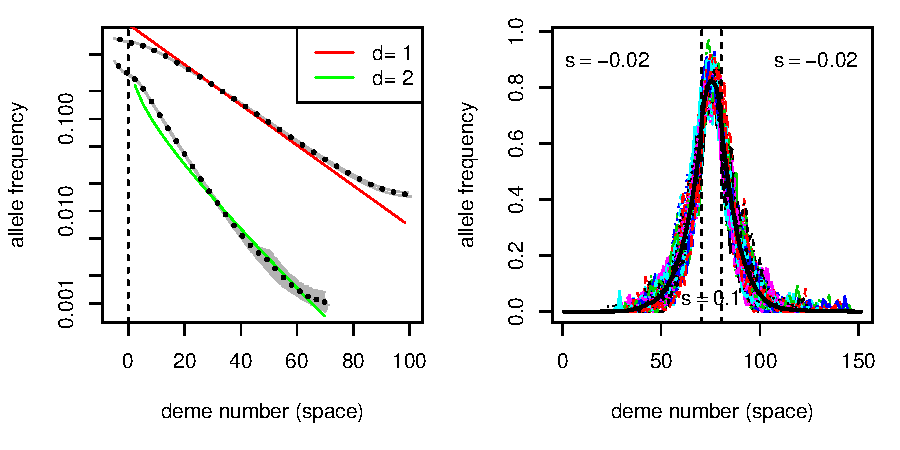
\includegraphics{sim-occupation-freqs}
  \end{center}
  \caption{
  \textbf{(A)} 
  Mean occupation frequencies of individual demes (grey dots)
  and averaged over demes at similar distances (black circles), on
  a one-dimensional grid of 201 demes, and
  a two-dimensional grid of $101\times 101$ demes.
  Superimposed in black is the decay predicted by \eqref{eqn:eqfreq},
  with $C$ chosen arbitrarily to give a reasonable fit.
  (The disagreement at long distances is due to boundary effects near the edge of the range.)
  \textbf{(B)} 
  Fluctuations: colored lines are snapshots of allele frequencies at evenly spaced times
  from a one-dimensional grid of 151 demes;
  the solid lines shows the cumulative mean occupation frequency across all generations.
  For both plots, the simulation was run for 1000 generations;
  the focal allele is beneficial in the central 20 demes, with $s_p=0.1$,
  and deleterious elsewhere, with $s_m=-0.02$; 
  demes had 1000 individuals in each;
  dispersal was to nearby demes with a mean dispersal distance of $\sigma \approx 1.66$  times the deme spacing.
   }   \label{fig:sim_occupation_freqs}
\end{figure}

This expected frequency $q(x)$ is the \emph{time-averaged} occupation frequency,
or in other words, the total number of $B$ alleles found across $T$ generations near location $x$, per unit area, divided by $T$.
If, for instance, $q(x)=.01$ and the population density is $\rho=10$ individuals per unit area, 
then in a survey tract of unit area around $x$ we expect to find one individual every 10 generations
-- or, perhaps more likely, 10 individuals every 100 generations.
This points to an important fact: 
close to the original patch, the ``equilibrium frequency'' $q(x)$ describes well the density of the $B$ allele at most times,
but far away from the patch, 
the equilibrium is composed of rare excursions of families of $B$
alleles, interspersed by long periods of absence. 
An example of one of these rare excursions is shown in Figure~\ref{fig:sim_snapshots}.
The relevant time scale on which $B$ alleles migrate between patches is given by the rate of appearance of such families.
To compute the rate of establishment by such migration,
we argue that these families (suitably defined) can be approximated by
independent branching processes whose spatial motion is described by Brownian motion.
Properties of these, combined with equation \eqref{eqn:eqfreq},
will lead us eventually to the expression \eqref{eqn:migrate} for the rate of effective migration,
an approximation that is valid if the distance $R$ is large (at least five times $\sigma/\sqrt{2s_m}$, say).

\begin{figure}[ht!]
  \begin{center}
    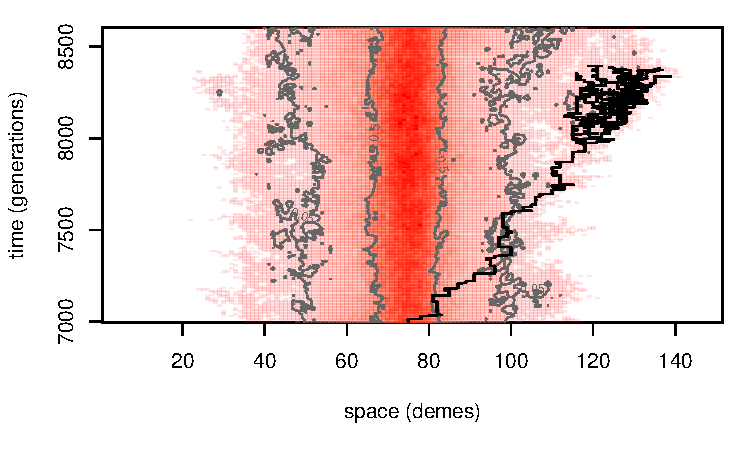
\includegraphics{sim-snapshots}
  \end{center}
  \caption{
  The temporal dynamics of the same simulation as Figure~\ref{fig:sim_occupation_freqs}B.
  A segment of the temporal dynamics: space is again shown across the horizontal axis;
  with time on the vertical axis; demes are colored darker red the greater then allele frequency at the corresponding time.
  The 50\% and 5\% frequency contour lines are in grey,
  and the genealogy of 50 individuals in a rare long-distance excursion is traced back with black lines.
  }   \label{fig:sim_snapshots}
\end{figure}

To make the argument, we decompose the genealogy of $B$ alleles into families in the following way.
First, consider the genealogy of all $B$ alleles that were alive at any time outside of the original patch.  
This is a collection of trees, each rooted at an allele living outside the patch whose parent was born inside the patch.
Next, fix some intermediate distance $r_0$ from the established patch,
and erase from the genealogy every allele that has no ancestors living further away than $r_0$ to the patch.
This fragments the original set of trees into a collection of smaller trees that relate to each other all $B$ alleles living outside of $r_0$ at any time,
and some living inside of $r_0$;
we refer to these trees as ``families''.
If $r_0$ is large enough that there are not too many families
and interactions between family members are weak,
then these families can be approximated by a collection of independent spatial branching processes
whose members are killed (actually, ignored) if they enter the original patch.
(This can be made formal in the limit of large population density, also taking $r_0$ large enough that the chance of reaching the original patch is small.)
This decomposition is illustrated in figure~\ref{fig:branching_decomp}.
In terms of these families, the equilibrium frequency above is then
\begin{align}
    \label{eqn:gestalt_q}
    \begin{split}
        q(x) &= \text{ ( outflux of families ) } \times \text{ ( mean occupation density of a family at $x$ ) } ,
\end{split}
\end{align}
and the quantity we wish to compute,
the effective rate of at which \emph{families of} migrant $B$ alleles establish in a new patch at distance $r$, 
is
\begin{align}
    \label{eqn:gestalt_migrate}
    \begin{split}
        \migrate(x) &= \text{ ( outflux of families ) } \times \text{ ( probability a family establishes in patch at $x$ ) }
    \end{split}
\end{align}
The quantities on the right-hand side depend implicitly on $r_0$.
All terms except the ``outflux of families'' are calculations with spatial branching processes;
and we can solve for this outflux using the established form for $q(r)$ in \eqref{eqn:gestalt_q}.
Note that $\migrate$ reflects the mean number of establishing migrant families per unit time, rather than individuals.

%%%%
\subsubsection{The genealogy of migrant families}

To understand the process of adaptation by migration,
we therefore need to look more closely at the rare families of $B$ alleles far from the patch where it is established.
Consider one such family,
that lives far from the original patch.
As noted above, we will model this by assuming that each individual
migrates, then reproduces, independently of all other family members.
The mean squared migration distance is $\sigma^2$, takes the migrant in a random direction,
and if migration takes the individual into a patch where the $B$ allele is favored, 
we drop the individual from our family.
Since the $B$ allele is uniformly deleterious elsewhere,
we can decouple reproduction and migration
by first forming a tree in which each individual has a random number of offspring
then recursively assigning spatial locations to each individual in the tree,
and finally pruning any branches that happen to wander into a patch.
By our definition of fitness, the mean number of offspring per individual is $\exp(-s_m)\approx 1-s_m$,
and the variance is $\xi^2$.
This pruning removes both branches leading back into the already established patch (which are irrelevant)
and branches leading into the new patch (we will need to count these).
Since we are concerned with the rare migrant families that transit quickly between patches, 
back migrants to the already established patch will contribute little, since they are going the wrong direction;
so to simplify the analysis we ignore this detail.  % but could add this detail in an appendix

Since each individual has on average $e^{-s_m}$ offspring,
the expected family size after time $t$ is $e^{t s_m}$.
Therefore, if we define $k_e(t)$ to be the chance that the family
has gone extinct by time $t$, 
%\plr{switched from $p_e(t)$ to $k_e(t)$ to not conflict with prob of estab.  better suggestion?}
and let $K_t$ be the (random) family size conditioned on nonextinction,
then by Bayes' rule, $e^{-s_m t} = (1-k_e(t))\E[K_t]$.
It turns out that if the distribution of offspring numbers is not too heavy-tailed \citep[see][for details]{jagers1975branching},
then $K_t$ has a limiting distribution: $K_t \dconv K$ 
and that $e^{-s_m t}/(1-k_e(t)) \to \E[K]$ as $t \to \infty$.
In other words, the chance of survival to time $t$ is a constant multiplied by $e^{-s_m t}$,
and conditional on survival, the family size is given by a fixed distribution.

This suggests that families can be well-described by motion of a central ``trunk'',
dies at a random time whose distribution is given by $k_e(t)$,
and conditional on survival of this trunk, the family is composed of side ``branches'' off of this trunk,
as depicted in Figure~\ref{fig:branching_decomp}.
We can understand this quite concretely, by a method described rigorously by \citet{geiger1999elementary} \citep[see also][]{chauvin1991growing}.
When we condition on survival until $t$, we condition on existence of
at least one ``trunk'' lineage surviving from time $0$ to time $t$ (the long red
lineage in Figure \ref{fig:branching_decomp}).
Given this lineage, nothing distinguishes any of the other reproduction events --
each individual along the trunk lineage must give birth to at least one offspring,
and all other reproduction events are unconditioned.
In other words, the genealogy of a family that survives until $t$
can be decomposed into a ``trunk'' that lasts until $t$
which sprouts independent ``branches'' that may or may not survive until $t$.
Concretely, if we write $Z_t$ for the number of offspring in the branching process alive at time $t$,
% (so $\P\{Z_t = 0\} = k_e(t)$),
then this gives the following decomposition:
\begin{align}
  \left( Z_t \; \vert \; Z_t>0 \right) \deq 1 + \sum_{s=0}^t \sum_{k=1}^{W_s-1} Z^{(s,k)}_{t-s},
\end{align}
where each $Z^{(s,k)}$ is an independent copy of $Z$ 
that arose from the main branch in generation $s$,
and each $W_s$ is an independent copy of the offspring distribution, conditioned on $W_s \ge 1$.


\begin{figure}[ht!!]
  \begin{center}
    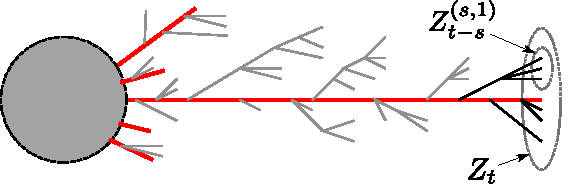
\includegraphics{branching-concept}
  \end{center}
\caption{Cartoon of the decomposition described in the text. 
Migrants families that get further than $r_0$ from the already-established patch (grey circle);
each is composed of a ``trunk'' lineage (in red), whose spatial motion we follow,
embellished by transient branches.
For the depicted long-lived family, these are further distinguished by those still alive at time $t$ (in black)
and those that did not survive until $t$ (in grey).
Figure~\ref{fig:sim_snapshots} has a depiction of such a family, from a simulation. 
Note that the spatial motions of lineages are independent random walks
(and hence should be much wigglier than in this cartoon).
} \label{fig:branching_decomp}
\end{figure}

This suggests that we add in the spatial motion by following only the motion of the ``trunk''
(i.e.\ the red line in figure \ref{fig:branching_decomp}),
whose motion is is approximately Brownian, with variance $\sigma^2$ per generation.
(Recall $\sigma$ is the dispersal distance.)
We can use these two ingredients, Brownian motion and a branching process, 
to compute the terms of equations \eqref{eqn:gestalt_q} and \eqref{eqn:gestalt_migrate}.


%%%%%%% %%%%%%%%%%%
\subsubsection*{Putting it together}

We are approximating the dynamics of the focal allele in the region further away than $r_0$ from the patch
as the sum of independent migrant families, each of whose dynamics are
given by a spatial branching process (as depicted in Figure \ref{fig:branching_decomp}).
Call $B(r_0)$ the region closer than $r_0$ to the patch, and $\partial B(r_0)$ its boundary.
Suppose that there is a constant outflux of migrant families from each point $x \in \partial B(r_0)$,
such that the long-term proportion of individuals near a point $x$ in $\partial B(r_0)$ that initiate new migrant families
is $\gamma(x)$.
To make expressions \eqref{eqn:gestalt_q} and \eqref{eqn:gestalt_migrate} more concrete,
we need to replace ``outflux of families'' by a sum over points at distance $r_0$ from the patch
of the outflux $\gamma$ at that point, multiplied by the relevant second quantity.
By examining the constituent terms,
it will turn out that equation \eqref{eqn:gestalt_migrate} 
is well-approximated by a constant multiple of \eqref{eqn:gestalt_q}.

First consider equation \eqref{eqn:gestalt_q} for the equilibrium frequency.
Suppose that $Z$ is one such spatial branching process as above, started at time 0 with a single individual at $x$,
defined so that $Z_t(A)$ is the number of descendant individuals alive at time $t$ living in the spatial region $A$.
The \emph{mean occupation density} of $Z$ can be thought of 
as the expected total number of offspring of a family beginning at $x$ that ever live at $y$.
Concretely, it is the density of $\E[\int_0^t Z_t(\cdot) dt]$,
i.e.\ the smooth function $u(x,y)$ that, integrated over a set $S$, 
gives the expected total number of individuals ever living in $S$:
\begin{align} \label{eqn:occupation_density_defn}
    \E\left[ \int_0^\infty Z_t(S) dt \right] = \int_S u(x,y) dy .
\end{align}
% Said another way, $u(x,y)$ is the expected number of offspring of a progenitor at $x$ that will ever be observed near $y$.
Since reproduction and spatial motion are independent,
$u(x,y)$ is the sum across all generations of the expected number of individuals alive in that generation,
multiplied by the probability density that spatial motion takes a lineage from $x$ to $y$,
i.e.\
\begin{align}
    u(x,y) = \int_0^t e^{-s_m t} p_t(x,y) dt .
\end{align}
The equilibrium frequency as decomposed in expression \eqref{eqn:gestalt_q} 
is the sum of mean occupation densities of a constant outflux of branching processes
from $\partial B(r_0)$:
\begin{align} \label{eqn:occupation_integral}
    q(y) &= \int_{\partial B(r_0)} \gamma(x) u(x,y) dx  . % \\
         % &= \int_{\partial B(r_0)} \gamma(x) \int_0^t e^{-s_m t} p_t(x,y) dt dx .
\end{align}

This form we can now compare to 
the expression \eqref{eqn:gestalt_migrate} for the outflux of successful migrants.
Consider the probability that a migrant family beginning with a single individual at $x$ will ever establish in the new patch,
which we assume is circular, has relatively small area $A$ and is centered at position $y$.
% The probability that this family reaches $A$ at time $t$ is the probability that it survives until $t$, $(1-k_e(t))$,
% multiplied by the probability that the family reaches the patch, given survival.
% If $t$ is large then as in the previous section, $(1-k_e(t)) \approx e^{-s_m t}/\E[K]$.
It would be possible to analyze directly the probability that a given migrant family establishes in the patch,
as in \citet{barton1987establishment};
but we make a simpler approximation, approximating this probability by the chance that the ``trunk'' hits the new patch,
multiplied by the chance that at least one member of the family escapes demographic stochasticity,
successfully establishing in the new patch.
Write $h_A(x,y)$ for the probability that the Brownian trunk
hits the new patch centered at $y$ before the family dies out,
and $f(A)$ for the chance that the family manages to establish in the new patch,
given that it successfully arrives.
As for $q(y)$ above, expression \eqref{eqn:gestalt_migrate} is properly an integral of $h_A(x,y)$:
\begin{align}\label{eqn:migrate_integral}
  \migrate(y) &= \rho \int_{\partial B(r_0)} \gamma(x) h_A(x,y) f(A) dx .
\end{align}

Intuitively, $h_A(x,y)$ counts each family once if it hits the patch,
while the occupation density $u(x,y)$ counts the total amount of time that the family spends in the patch.
Since the expected total time spent in the patch does not depend on the distance at which the family started
if we know that it survived to hit the patch,
it is intuitively reasonable that $u(x,y)$ and $h_A(x,y)$ are simply related.
Following this intuition,
and that $(1-k_e(t)) \approx e^{-s_m t}/\E[K]$,
it turns out (see Appendix~\ref{apx:hitting_occupation}) that
\begin{align} 
  h_A(x,y) \approx \frac{ g(A) }{ \E[K] } u(x,y),
\end{align}
where $g(A)$ is the total expected occupation time of the patch given the family arrives,
and recall that $\E[K]$ is the expected family size after a large number of generations, given survival.
Since the integrands in expressions \ref{eqn:occupation_integral} and \ref{eqn:migrate_integral} only differ by a factor
that (at least asymptotically) does not depend on the distance between $x$ and $y$,
we can obtain the migration rate by multiplying the equilibrium frequency by this factor.
The probability $f(A)$ that the family does not die out once it arrives at the new patch is
$\E[1-(1-p_e)^K] \approx 2 s_p \E[K] / \xi^2$,
if each member arriving has chance $p_e$ of establishing, independently.
% If we let $w$ be the width of the patch, then the remaining term is
% \begin{align}
%   s(w) \simeq \frac{1}{2s_m} \left( 1 - \left( \frac{\pi w \sqrt{2 s_m}}{ 2 \sigma } \right)^{\frac{d-1}{2}} e^{-w \sqrt{2s_m}/\sigma} \right).
% \end{align}
Combining with expressions for $g(A)$ in Appendix~\ref{apx:hitting_occupation},
we obtain that
\begin{align}
  \label{eqn:migrate} 
  \migrate(y) &\approx q(y) \times \frac{ \rho s_p  }{ \xi^2 s_m }  \\
  % \left( 1 - \left( \frac{\pi w \sqrt{2 s_m}}{ 2 \sigma } \right)^{\frac{d-1}{2}} e^{-w \sqrt{2s_m}/\sigma} \right).
  &\approx C \frac{ \rho s_p  }{ \xi^2 s_m } \left( |x| \sqrt{2 s_m}/\sigma \right)^{-(d-1)/2} \exp( - |x| \sqrt{2 s_m} / \sigma) .
\end{align}
This does not depend on $A$, because although
$f(A)$ and $g(A)$ in principle depend on the patch size (and geometry),
the dependence is very weak:
for instance, the width of a circular patch only very weakly affects the chance 
of establishment of a new migrant that appears on its edge,
as long as the patch is large enough.
For more discussion, including an expression for the outflux of migrants $\gamma(x)$, see Appendix~\ref{apx:hitting_occupation}.


%%%%%%%%%
\subsection{The probability of parallel adaptation between patches.} 
\label{ss:probparallel}

We now turn to the question of whether the separated populations adapt by parallel genetic changes 
or by the spread of a migrant allele between the patches
(or both, or neither).
As only a single mutation is required for individuals to adapt to the
poor habitat patch, subsequent mutations that arise after an allele becomes established in the patch gain no selective benefit. 
Similarly, an allele introduced into a patch by migration will not be favored by selection to spread, 
if the patch has already been colonized. 
Therefore, mutations selectively exclude each other from patches, over short time scales, 
and will only slowly mix together over longer time scales by drift and migration,
an assumption we also made in \citep{ralph2010parallel}. 
In reality, different mutations will likely not be truly selective equivalent,
in which case this mixing occurs over a time-scale dictated by the difference in selection coefficients.

We will assume that once a $B$ allele is introduced (by migration or mutation) and successfully begins to establish,
it becomes established in the poor habitat patch rapidly. 
Under this approximation, and the ``selective exclusion'' just discussed,
after one of the patches becomes colonized by a single $B$ allele, 
the other patch will become colonized by migration or mutation, but not by both. 
As such, the question of how the the second patch adapts
simply comes down to whether a new mutation or a migrant allele is the first to become established in the second patch. 
To work out how adaptation is likely to proceed, 
we can compare expressions \eqref{eqn:mutrate} and \eqref{eqn:migrate} above
for the effective rates of adaptation by new mutation and by migration.

The first thing to notice is that effective migration and mutation rates will be on the same order if 
$A \mu \approx (1/s_m) \exp(- R \sqrt{2 s_m} / \sigma)$,
where recall that $R$ is the distance between the patches,
and $A$ is the area of the not-yet-adapted patch.
In other words, the migrational analogue of ``mutational influx'' ($\mu \rho A$) 
is $\rho (1/s_m) \exp(- R \sqrt{2 s_m} / \sigma)$,
which depends fairly strongly on the selective disadvantage $s_m$ between patches.
Equivalently, the rates are roughly equal if
$R/\sigma = \log(1/(s_m A \mu))/\sqrt{2s_m}$,
which gives the critical gap size past which adaptation will be mostly parallel
in terms of selection coefficients, patch size, and mutation rate.

% ss <- 10^(-(1:6))
% log(1/ss)
% 1/sqrt(2*ss)
% sm <- .05; (-log(c(1e-3,1))-log(sm))/sqrt(2*sm)
% sm <- .001; (-log(c(1e-3,1))-log(sm))/sqrt(2*sm)
% (7+log(1/ss))/sqrt(2*(ss))
% (7+log(1/(.5*ss)))/sqrt(2*(.5*ss))

\gc{NOT SURE IF ANYONE HAS LOOKED AT THI IN LONG TIME?}
If we take the mutational influx in a patch to be one per 1,000 generations ($\rho A \mu = .001$)
and the population density to be 1 ($\rho =1$, so $\log(A\mu)\approx 7$)
then adaptation is mostly parallel for patches separated by gaps larger than $R/\sigma > (7+\log(s_m))/\sqrt{s_m}$.
If the selective pressure is fairly strong (say, $s_m=.05$),
then for migration to be slower than mutation,
the distance between patches must be at least 30 times the dispersal distance (i.e.\ $R/\sigma > 30$).
If $s_m$ is much smaller, say $s_m = .001$, 
then the patches must be separated by several hundred times the dispersal distance (i.e.\ $R/\sigma > 300$).
The situation does not change much if the influx is quite a bit higher -- even if $A \mu = 1$ (so $\log(A\mu) \approx 2.3$),
the required separation between patches is only reduced to $R/\sigma > 10$ with $s_m=.05$ and $R/\sigma>150$ for $s_m=.001$.
On the other hand, if the separation is much smaller than this transitional value, 
then adaptations are likely to be shared between patches.

One way to visualize this is by a phase diagram.
In figure \ref{fig:phase_diagram},
we give a contour plot for the time until adaptation by migration ($\Tmig = 1/\migrate$) and by new mutation ($\Tmut=1/\mutrate$)
as a function of various parameters. 
This gives us an idea of not only the parameter space where parallel adaptation is likely ($\Tmig \ll \Tmut$),
but also where adaptation by any means takes a very long time ($\Tmig$ and $\Tmut$ both very large),
and important check in applications.

\begin{figure}[ht]
  \begin{center}
    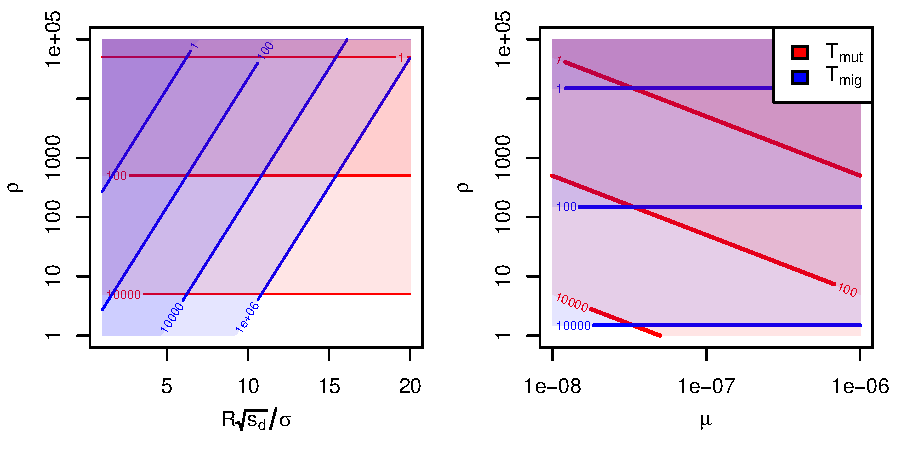
\includegraphics{phase-diagram-log}
  \end{center}
  \caption{
  Shaded contour plots of
  mean time until adaptation in a new patch occurs by migration ($\Tmig$, blue) or by mutation ($\Tmut$, red),
  as a function of population density ($\rho$), 
  distance to an already adapted patch in units of dispersal distance ($R/\sigma$),
  strength of deleterious selection ($s_m$),
  and mutation rate scaled by patch area ($\mu A$).
  The black, dotted line shows values where $\Tmig=\Tmut$.
  Default parameter values were $A=100$, $\rho=10$, $\mu=10^{-8}$, $s_p=0.1$, $s_m=0.01$, $R/\sigma=50$, and $\xi^2=1$.
  Note that population density and mutation rate are shown on a log scale.
  \label{fig:phase_diagram}
  }
\end{figure}

Taking these approximations at face value, 
and assuming both rates are small, 
the time until the first of the two patches is colonized by the $B$
allele will be approximately exponentially distributed with mean $1/(2
\mutrate)$.
Following this, the time until the second patch is subsequently colonized 
(via either migration or new mutation) 
will be exponentially distributed with mean $1/(\mutrate+\migrate)$.
Both these rates scale linearly with population density ($\rho$) 
and the probability of establishment of a rare allele ($p_e\approx 2 s_b/\xi^2$),
so that the overall time to adaptation is robustly predicted to increase with offspring variance ($\xi^2$)
and decrease with population density and benefical selection coefficient.
Furthermore, the probability that the second adaptation is a new mutation,
i.e.\ the probability of parallel adapatation, is 
\begin{equation} \label{eqn:parallel_prob}
  \frac{\mutrate}{\mutrate+\migrate(r)} = \frac{ A \mu s_m }{2 A \mu s_m + \left(r \sqrt{2 s_m} /\sigma \right)^{-(d-1)/2}\exp\left(- \sqrt{2 s_m} r / \sigma \right) },  
\end{equation}
so that the probability of parallel mutation should increase
approximately logistically with the distance between the patches, at rate $\sqrt{s_m} /\sigma$. 


%%%%%%%%%%%%
\subsubsection{Multiple patches}
Above we worked with two patches separated by distance $R$;
but these calculations apply as well to multiple patches
in which the $B$ allele can facilitate local adaptation. 
Under our assumptions of mutational exclusion and rapid establishment, 
each patch will adapt through establishment of a single copy of the $B$ allele, 
either by migration or mutation.
If we imagine that the times between successive establishments is the result of many nearly-independent attempts
with small probability of success,
the process of occupation is well approximated by a Markov chain,
whose state records the labeling of patches according to the colonizing allele
(or none, for those that haven't yet adapted).

If not yet adapted, a patch of area $A$ will acquire the adaptation by new mutation at rate $2 s_p \mu \rho A/\xi^2$ (equation \eqref{eqn:mutrate}).
Suppose that patches $1, \ldots, k$ are already adapted,
and that these patches are at distances $r_1, \ldots, r_k$ away from this unadapted patch.
The total rate of adaptation through migration, from equation \eqref{eqn:migrate}, is
\begin{equation}
  \migrate(r_i) = C \frac{ \rho s_p }{\xi^2 s_m} \sum_{i=1}^{k} \left(r_i \sqrt{2 s_m} /\sigma \right)^{-(d-1)/2} \exp\left(- r_i \sqrt{2 s_m} /\sigma\right),
\end{equation}
and if the patch adapts through migration, the probability the adapted allele 
comes from patch $i$ is 
\begin{align}  
  \frac{\left(r_i \right)^{-(d-1)/2} \exp\left(- r_i \sqrt{2 s_m}
  /\sigma\right)} {\sum_{j=1}^{k}  \left(r_i \right)^{-(d-1)/2} \exp\left(- r_i \sqrt{2 s_m}
    /\sigma\right) } .
\end{align}
These specify the transition rates of the process.

Since the compound parameter $s_p \rho / \xi^2$ is common to both rates,
it functions only as a time scaling of the process, 
and therefore has no effect on the final configuration, namely, 
the sets of patches sharing the genetic basis of their adaptive response.

Also note that we can rescale time by the typical patch size, and introduce a parameter, say $a_k = A_k/\bar A$,
making the properties (other that the time scaling) of the discrete model independent of the \emph{numerical sizes} of the demes themselves.
This is complementary to the results of \cite{softsweepsII}, who showed that multiple mutations are likely to arise \emph{within} a panmictic deme
if the population-scaled mutation rate $2 N \mu$ is greater than $1$.

The resulting discrete process is quite general,
but if we oversimplify back to the island model, it is tractable:
suppose the probability of adaptation by mutation is the same for each patch
and by distance is the same for each pair of patches.
The resulting process is a continuous-time version of the ``Chinese restaurant process''
described in \citet{aldous1985exchangeability} and \citet{pitman1995partitions},
and so the final partition of types across demes has the Ewens
sampling distribution with parameter $A \mu s_m/ \exp (-sqrt{2 s_m}r/\sigma)$.
Now we can compute most properties we might want about the process.
For instance, the proportion of demes that shares the same origin as a randomly sampled deme
is approximately Beta distributed -- see \cite{donnelly1989continuity} and \cite{perman1992sizebiased}.
The high connectedness of the discrete deme island model means that the expected number of distinct alleles
grows with the $\log$ of the number of demes, 
which strongly contrasts with the continuous spatial model 
where the local nature of dispersal means that doubling the species range will double the number of mutations expected. 


\begin{figure}[ht]
  \begin{center}
    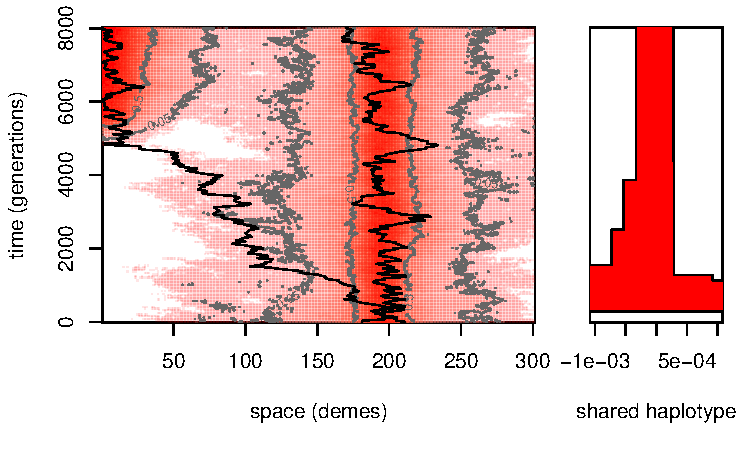
\includegraphics{sim-transit.pdf}
  \end{center}
  \caption{
  \textbf{Adaptation by migration:}
  An initially unadapted patch (10 demes at the left end of the range) is colonized around generation 5000;
  a representative lineage from the new patch is shown transiting between the two and coalescing with a lineage
  in the unadapted patch.
  In the left panel, as in Figure~\ref{fig:sim_snapshots}, color and contours show allele frequency across space and time;
  other simulation parameters are as in Figures~\ref{fig:sim_occupation_freqs}B and \ref{fig:sim_snapshots}.
  The right panel shows (in red) the length of the shared haplotype between the two lineages
  around the selected locus,
  which decreases as time progresses.
  \label{fig:lineagesmotion}
  }
\end{figure}




%%%%%%%%%
\subsection{Length of the hitchhiking haplotype}
\label{ss:haplotype_length}

If a patch adapts through new mutation or a rare migrant lineage, the
genomic region surrounding the selected site will hitchhike along with it \citep{maynardsmith1974hitchhiking},
so that at least initially, all adapted individuals within a patch
share a fairly long stretch of haplotype. 
Pairs of individuals within a patch will share a haplotype of mean genetic length of
about $\log(\rho A s_p)/s_p$ around the selected site, 
as long as the patch is reasonably well mixed by dispersal
\citep[otherwise see][]{barton2013genetic}.
This association gets slowly whittled down by recombination during interbreeding at the edge of the patch;
but there will always be longer LD nearby to the selected site. 

When an already adapted patch colonizes another through migration,
then the newly colonized patch will inherit a long piece of haplotype around the selected site from the originating patch.
The genetic length of this haplotype is roughly inversely proportional to the
number of generations the allele spends ``in transit'', 
because each reproductive event in locations where the allele is at
low frequency will likely recombine haplotypes of the $b$ allele closer to the adaptive allele. 
In this case, the haplotype is literally hitchhiking across geography!
Figure~\ref{fig:lineagesmotion} shows a simulation of such an event,
including the lineage that founds an adaptive population on a second patch,
and the length of the haplotype shared between this lineage and one in the original patch.
The entire time that the lineage is outside the region where the $B$ allele is common (dark red in Figure~\ref{fig:lineagesmotion}), 
the haplotype that accompanies it is broken down rapidly. 
After the lineage establishes on the patch, the rate of decay of the haplotype is slowed significantly, 
since most others with which it recombines have similar haplotypic backgrounds. 
We first discuss the transit of the lineage, and its accompanying haplotype, and return
to how haplotypes are whittled down within estalbished patches in the next section.


Above we argued that a good model for this transit is a single Brownian trunk lineage
surrounded by a cloud of close relatives of random size $K$
whose chance of surviving until $t$ generations is $1-k_e(t)$.
Consider a single such family, and let $\tau$ be the (random) time at which it first hits the new patch,
with $\tau = \infty$ if it never does. 
We assume that the length of the hitchhiking segment depends only on 
the time spent by the trunk lineage of the first successful migrant ``in transit'' between the patches,
i.e.\ $\tau$ conditioned on $\tau < \infty$.
In so doing, we neglect 
recombination between $B$ alleles (since they are at low density in transit, we assume this is rare),
and the possibility that more than one migrant family is in transit at once
(so that faster migrants would be more likely to have arrived first);
but these factors should be minor if the rest of our framework fits.

Our first obstacle is that we do not know $1-k_e(t)$, 
the probability a family survives until $t$, exactly.
However, we do know that $1-k_e(t) \simeq e^{-s_m t} / \E[K]$,
i.e.\ that it has exponential tails.
Since $\E[K] \approx 1/s_m$, it is sensible to make one further approximation,
replacing this random time by an exponential with rate $s_m$.
Once we do this, 
we can use standard results on hitting times of $d$-dimensional Brownian motion
that is killed at rate $s_m$ \citet[][(2.2.0.1 and 4.2.0.1)]{borodin2002handbook} 
In particular, if the patch is circular with radius $w$ and a distance
$R$ from the already adapted patch, then 
we know that the Laplace transform of the transit time $\tau$ is
\begin{align}
  \E[e^{-\ell \tau}] &=
    \begin{cases}
      e^{- R \sqrt{2(s_m+\ell)}/\sigma} \qquad & d=1 \\
      \frac{ K_0( (R+w)\sqrt{2(s_m+\ell)}/\sigma) }{ K_0( w\sqrt{2(s_m+\ell)}/\sigma) } \qquad & d=2  ,
    \end{cases} \label{eqn:borodinresult}
    % &= \left( R/w +1 \right)^{-\frac{d-1}{2}} e^{- R \sqrt{2(s_m+\ell)}/\sigma}  (1+O(1/w)) .
\end{align}
where $K_0$ is a modified Bessel function of the second kind.
We are interested in lineages that manage to reach the patch before being killed,
i.e.\ having $\tau < \infty$,
which occurs with probability
$\P\{\tau < \infty\} = \lim_{\ell \to 0} \E \left[\exp(-\ell \tau) \right]$. 

To keep the expressions simple, in the remainder of this section we only compute quantities for one dimension.
By Bayes' rule, the Laplace transform of $\tau$ for a successful lineage is
\begin{equation} \label{eqn:haplen_cdf}
\E[e^{-\ell \tau}|\tau<\infty]  = \exp\left\{{-\frac{R}{\sigma}\left(\sqrt{2(\ell+s_m)} - \sqrt{2s_m}\right)}\right\} .
\end{equation}
This can be differentiated to find that the expected transit time is
\begin{equation} 
  \E[\tau] = (R\sqrt{2s_m}/\sigma)\times 1/(2s_m) \label{eqn:mean_tau}
\end{equation}
and that $\var[\tau] = (R\sqrt{2s_m}/\sigma) \times 1/(2s_m)^2$.

% \simeq (R/w+1)^{-(d-1)/2} \exp(- R \sqrt{2s_m}/\sigma)$.

% Above, we approximated this by the time $\tau$ it takes the trunk lineage to hit the new patch;
% now that we are studying a successful migrant family means we need to condition on the establishment occurring, i.e.\ on $\tau < \infty$.
% By the above arguments, and equation~\eqref{eqn:estab_prob}, we have that the conditional probability density is
% \begin{align}
%   \P\{\tau\in dt | \tau<\infty \} &= \frac{\P\{\tau \in dt\}}{\P\{\tau<\infty\}} \\
%   &= \frac{R}{\sigma^3 t^{3/2}\sqrt{2\pi}} \exp\left(-\frac{R^2}{2t\sigma^2} -s_m t + \sqrt{s_m} \frac{R}{\sigma} \right) .
% \end{align}
% \plr{more dimensions}

Since each generation spent in transit provides an opportunity for recombination,
if recombination is Poisson, the length of the haplotype (in Morgans)
initially shared between populations on each side of the selected locus is exponentially distributed
with mean $\tau$, so that if $L$ is the length of hitchhiking segment on, say, the right of
the selected locus, then
\begin{equation} \label{eqn:haplen_cdf2}
\P\{L>\ell\} = \E[e^{-\ell \tau}|\tau<\infty] ,
%  &= \exp\left\{{-\frac{R}{\sigma}\left(\sqrt{2(\ell+s_m)} - \sqrt{2s_m}\right)}\right\} .
\end{equation}
and so (one minus) equation~\eqref{eqn:haplen_cdf} in fact gives the cumulative distribution function of $L$.
The form of this distribution function implies that if $Y$ is an exponential random variable with rate $R\sqrt{2}/\sigma$,
then $L$ has the same distribution as $(Y + \sqrt{s_m})^2 - s_m$.
Furthermore, the expected length of shared hitchiking haplotype is
\begin{equation} \label{eqn:haplotype_length}
\E[L] = \sigma \sqrt{2s_m}/R + \sigma^2/R^2
\end{equation}
and $\var[L] = 2s_m\sigma^2/R^2 + 4 \sigma^3 \sqrt{2s_m}/R^3 + 5 \sigma^4 / R^4$.
For two dimensions, asymptotics of Bessel functions show that $L$ has the same tail behavior;
but how other properties might change is unclear. 

As a general rule of thumb, equation~\eqref{eqn:mean_tau} means that families who successfully establish
move at speed $\sqrt{s_m} \sigma$ towards the new patch 
-- if $s_m$, the strength of the selection against them, is smaller, the need to move quickly is less imperative.
Then, equation~\eqref{eqn:haplotype_length} means that the haplotype length
is roughly the length one would expect given the mean transit time.
Note that we have become used to seeing $\sigma$ divided by $\sqrt{s_m}$, rather than multiplied;
it appears here because $\sigma/\sqrt{s_m}$ is a length scale, 
and to convert it to a time this is divided by $1/s_m$.
This intuitive picture can be expanded by a central limit theorem:
for large $R$, the deviation of $\tau$ about its mean is asymptotically Gaussian,
and the haplotype halflength $L$ is exponential.

% In Appendix~\ref{apx:limiting_dist_of_HH_haplotype}, 
% we also give some expressions for the limiting distribution of the length of shared haplotype.

% 
% \section{Limiting distribution of the transit time and hitchhiking haplotype}
% \label{apx:limiting_dist_of_HH_haplotype}
% 
% In the above we already assumed that the inter-patch distance $R$ is large relative to the migration-selection cline width $\sigma/\sqrt{s_m}$;
% also taking the large-$R$ limit, obtains a more intuitive description of the process
% via a central limit theorem for $\tau$.
% Define $\eta_\tau$ to be the deviation of $\tau$ from its mean, normalized by its standard deviation,
% so that $\tau = R/\sigma(2s_m)^{-1/2} + \eta_\tau \sqrt{R/\sigma} (2s_m)^{-3/4}$.
% Plugging this into equation~\eqref{eqn:haplen_cdf},
% after some algebra (and using that $\sqrt{R+\epsilon} = \sqrt{R} + \frac{\epsilon}{2\sqrt{R}} - \frac{\epsilon^2}{2\sqrt{R}^3} + O(\epsilon^3)$) we obtain that
% \begin{align}
%   \E[e^{-\ell \eta}] &= \exp\left\{ \frac{\ell^2}{2} + O\left(\frac{1}{R}\right) \right\}.
% \end{align}
% Since the Laplace transform uniquely determines a distribution \citep{durrett1996probability},
% this implies that $\eta_\tau$ converges in distribution to a standard Gaussian random variable as $R \to \infty$.
% In other words, we now know that the distribution of $\tau$ about its mean is approximately Gaussian.
% Since the standard deviation of $\tau$ is of lower order than its mean,
% a similar calculation shows that for large $R$, the haplotype halflength $L$ is approximately exponentially distributed, 
% with mean $\sqrt{2s_m} \sigma/R$.



% \begin{align}
%   \E[e^{-\ell \eta}] &= \E\left[ \exp\left\{-\ell\left(\tau - \frac{R}{\sigma\sqrt{2s_m}}\right)\frac{(2s_m)^{3/4}\sqrt{\sigma}}{\sqrt{R}} \right\} \right] \\
%   &= \E\left[ \exp\left\{ - \left(\frac{\ell (2s_m)^{3/4} \sqrt{\sigma}}{\sqrt{R}}\right) \tau \right\} \right] \exp\left( (2s_m)^{1/4} \sqrt{\frac{R}{\sigma}} \right) \\
% \end{align}



%%%%%%% %%%%%%%%%%
\subsection{Length of the shared haplotype within a patch}
\label{ss:patch_haplotype}

The other key issue in thinking about the population genetic signal of adaptation in spatial patches 
is the process by which haplotypes are whittled down within patches, 
which plays into a number of aspects of haplotype sharing. 
The initial haplotype that sweeps within a patch 
will be dispersed over time by recombination;
likewise, the haplotype that is shared between patches coadapted by migration
(equation~\ref{eqn:haplotype_length}) will also break down. 
We first develop a simple approximation to the rate 
at which recombination breaks down haplotypes within patches. 
If we wait long enough after the initial adaptation of a patch,
the haplotype that swept initially will have decayed due to this process of recombination. 
However, we may still expect to find individuals within the patch sharing long haplotypes around the selected locus
than with individuals elsewhere,
since selection against migrants 
decreases mean coalescence times within the patch near the selected locus.
%\citep{bartonpaper,charlesworths}. 

Refer again to Figure~\ref{fig:lineagesmotion}. 
When a lineage is in a region with high frequency of $B$ alleles (dark red), 
it is very unlikely to recombine off the $B$ background. 
However, when it wanders out of the patch,
into regions with lower frequency of $B$ alleles,
when it recombines it will
usually be on to the background of the $b$ allele.

A detailed treatment of this is well beyond the scope of this paper,
but we can get a good idea of the genomic scale of these effects through heuristic arguments.
To understand the probability of a recombination moving our lineage
off of the B background we need to understand what fraction of the
time our lineage spends in geographic regions where $b$ is common. 
Consider the lineage of a single $B$ allele, moving back through time,
in a patch at migration-selection balance, 
i.e.\ with the local proportion of $B$ alleles near $x$ equal to $p(x)$,
and suppose that the lineage stays close enough to the patch 
that fluctuations about $p(x)$ are small. 
(Note that this assumption differs from
previous sections, but here our focus is on a typical lineage in the
patch rather than the rare lineages that make it far from the patch).
If we suppose that type $B$ individuals at location $y$ reproduce at rate $1+s(y)$,
and the chance their offspring move to $x$ is $m(y,x)$ (with $\sum_x m(y,x)=1$),
then the total rate of influx of $B$ alleles from $y$ into $x$ is $\rho p(y) (1+s(y)) m(y,x)$.
As argued by \citet{hudson1988coalescent}, the rate at which a $B$ lineage moves from $x$ to $y$
is this influx divided by the local abundance of $B$ alleles,
or $p(y) (1+s(y)) m(y,x) / p(x) $.
After the same large-population, continuous-space limit that underlies the rest of this paper (Appendix~\ref{apx:eqfreq}),
this motion should converge to a diffusion process \citep[as assumed by e.g.][]{hallatschek2008surfing},
notwithstanding some technical difficulties (e.g.\ discontinuity of $s(x)$).
This diffusion, when at $x$, 
is pulled toward regions with more $B$ alleles
by a drift term $(1+s(x))\frac{d}{d\,x} \log( p(x) (1+s(x)) )$,
where $s(x)=s_p$ if $x$ is in the patch and $s(x)=s_m$ otherwise, 
and moves at speed $\sqrt{1+s(x)}$ (which is nearly constant, since $s(x)$ is small).
In It\^o differential notation, 
the location $X_t$ of a $B$ lineage $t$ generations ago satisfies
\begin{align}
    d X_t &= (1+s(X_t)) \frac{d}{dx} \log( p(X_t) (1+s(X_t)) ) dt + \sigma \sqrt{1+s(X_t)} dB_t,
    % &=  ( \log(p(X_t))' (1+s(X_t)) + s'(X_t) ) dt + \sqrt{1+s(X_t)} dB_t,\\
\end{align}
where $B_t$ is a standard Brownian motion.
Furthermore, it is easy to verify that the stationary distribution of this process has density
\begin{align}
  \pi(x) = \frac{ p(x)^2 (1+s(x)) }{ \int_y p(y)^2 (1+s(y)) dy } . \label{eqn:lineagestatdist}
\end{align}
A lineage at a locus at genetic distance $r$ that begins linked to a $B$ allele
moves as a $B$ lineage up until the most recent time
it recombined from a $b$ background to a $B$ background,
which occurs when at $x$ with rate $r (1-p(x)) (1+s(x)/2)$.
The Feynman-Kac formula could then be used to write down differential equations
solved by various moments of the haplotype length as a function of the sampling location of the lineage;
instead, we only use the above as a guide for rough approximation.

Based on this picture of
the lineage bouncing around in the patch,
we propose a simple heurstic to describe the probability of recombination. 
If recombination is on a slower time scale than mixing within the patch,
then the time until the last recombination is the integral of $r (1-p(x)) (1+s(x)/2)$ 
against the stationary distribution (equation~\ref{eqn:lineagestatdist}).
Within the patch, $p(x) \approx 1$,
so recombination off the $B$ background is unlikely to occur,
and so the rate of recombination depends to a first approximation 
on the proportion of the patch in which $p(x)$ is intermediate,
i.e.\ where both $B$ and $b$ are present.
This region where $p(x)$ is intermediate has width of order $\sigma/\sqrt{s}$, where $s = \min(s_p,s_m)$.
As we increase the size of a patch, the area on which $p(x)$ is intermediate scales with the perimeter of the patch.
Therefore, the proportion of the time a lineage at stationarity is found in the intermediate regions
multiplied by $p(x)$ in these intermediate regions, where we assume
$p(x) \approx 1/2$. Under these approximations the per generation rate of
recombination of a linked lineage to the $b$ background is
reduced by a factor roughly equal to the proportion of the patch lying within distance $\sigma/\sqrt{s}$ of the boundary,
so the effective recombination rate is
% \plr{Note to ourselves: If a $d$-dimensional object with area A has radius $r$ (in any sense)
% and you shrink it to have radius $r_0$,
% then the resulting object has area $A \times (r_0/r)^d$;
% here we have $r_0 = r - \sigma/\sqrt{s}$,
% in $d=1$ the radius is $A/2$ and in $d=2$ it is $\sqrt{A/\pi}$.}
\begin{align}
r_\text{eff} &=
    \begin{cases}
    r \frac{ \sigma /\sqrt{s} }{ \sigma/\sqrt{s} + A }    \qquad & d=1 \\
   r \frac{\pi  \sigma /\sqrt{s}  \left( \sigma /\sqrt{s}+
  \sqrt{A/\pi} \right)}{A+\pi \sigma/\sqrt{s} \left( \sigma/\sqrt{s} +
  \sqrt{A/\pi} \right) }    \qquad & d=2 ,  
\end{cases}
\label{eqn:rec_rate_within}   %(\sigma/\sqrt{s})A^{-1/d}
\end{align}
so that $T$ generations after the founding of a patch we expect a
haplotype of genetic length $1/(r_\text{eff}T)$ Morgans to remain linked to
the $B$ allele in a typical lineage. 
Note that the length of haplotype
decays at a rate roughly proportional to $\sqrt{s}/ \sigma$, as the narrower the cline the less
opportunity for recombination to move our lineage off the $B$ background. 
 

 
Finally we can consider the expected length of haplotype shared within a patch. 
To do this, we compare the rate of recombination between $B$ and $b$ haplotypes (equation~\ref{eqn:rec_rate_within})
to the rate of coalescence of $B$ haplotypes within a patch. 
We will assume that mixing within the patch is fast compared to the rate of drift, 
so that the rate of coalescence of $B$ alleles within a patch is 
$\xi^2/(A\rho)$,
the ``variance effective population size'' of the patch
(this bypasses the well-known difficulties to spatial coalescence \citep{felsenstein1975pain,barton2002neutral}).
The rate of recombination and coalescence will be on the same order if
$\xi^2 /(A\rho) \approx r (\sigma/\sqrt{s}) A^{-1/d}$, 
and hence the genetic length of haplotype shared between pairs of
individuals within the patches at equilibrium is on the order of
\begin{align} \label{eqn:within_haplotype_length} 
  r = \frac{\sqrt{s} \xi^2}{\sigma \rho A^{(d-1)/d}} 
\end{align}
which does not depend on $A$ in one dimension,
but decreases with $\sqrt{A}$ in two dimensions.
In applications, this can be compared to equation~\eqref{eqn:haplotype_length}
for the length of shared haplotype between patches.

%%%%%%%%%%
\subsection{Applications} 
\label{ss:applications}
% FOR REFERENCE:
% On Wed, May 28, 2014 at 10:20 AM, Michael Nachman <mnachman@berkeley.edu> wrote:
% > Graham:
% >
% > The density is probably in the range of 10-40 animals per hectare (10,000
% > m^s).  We built enclosures of 0.25 hectare and found that they could support
% > about 10 animals with food provided ad libitum, so I think this is an upper
% > density (i.e. 40/hectare).  As for dispersal distance, I'm less sure.
% > Studies on closely related species (genus Perognathus) in similar habitats
% > suggest distances of 100's of feet.  Attached are some old papers that tried
% > to estimate dispersal distances in Perognathus.
% > best,
% > Michael

Hoekstra, Nachman, and colleagues have made an extensive study of coat color in the rock pocket mouse, 
\emph{Chaetodipus intermedius}, building on classic work by
\citet{benson1933concealing}, \citet{DiceBlossom1937} and \citet{dice1940ecologic}.
These mice live on rocky outcrops throughout the southwestern United States and northern Mexico, 
and generally have a light pelage similar to the predominant rock color.
However, in some regions these mice live on darker substrates (e.g.\ old lava flows),
and in these patches have much darker pigmentation, 
presumably to avoid visual predators.
\citet{nachman2003genetic} demonstrated that on one of these flows (Pinacate), 
much of the change in coloration is due to an allele at the MC1R locus.
This dark allele differs from the light allele by four amino acid changes, 
and has a dominant or partially dominant effect depending on the measure of coat color assessed. 
These areas of dark rock are separated from each other by a range of distances, 
with some being separated from any other by hundreds of kilometers of light colored substrate. 
The Pinacate allele is not present in a number of other populations of dark colored rock pocket mouse, 
suggesting these populations have adapted in parallel \citep{nachman2003genetic ,hoekstra2003different}.
However, there is some evidence \citep{hoekstra2004local} that, elsewhere in the range, 
multiple dark outcrops may share a dark phenotype whose genetic basis has been spread by migration
despite intervening light habitat. 
We apply our theory to this example,
in particular investigating how the probability of parallel mutation depends on 
the distance between lava flow patches.

A key parameter above was the dispersal distance divided by the square root of strength of selection against the focal allele between patches, $\sigma/\sqrt{s_m}$. 
\citet{hoekstra2004ecological} studied the frequency of the dark MC1R allele and coat color phenotypes, 
at sites across the (dark) Pinacate lava flow and at two nearby sites in light-colored rock.
On the lava flow the dark MC1R allele is at 86\% frequency,
while at a site with light substrate 12km to the west (Tule), the frequency is 3\%.
The dark allele was entirely absent from Christmas pass, a site with light substrate 7km north of Tule, and 3km further from the lava flow.
In the other direction, the dark MC1R allele was at 34\% at a site with light substrate 10km to the east of the flow (O'Neill).
These numbers give us a sense of a plausible range of characteristic lengths.
Assuming the dark allele is at 50\% frequency at the edge of the lava flow, 
we can fit formula \eqref{eqn:eqfreq} to these frequencies
\citep[similar to][]{hoekstra2004ecological}.
Doing this for Tule we obtain $\sigma/\sqrt{s_m} \approx 3$km, 
and for O'Neill, $\sigma/\sqrt{s_m} \approx 30$km, giving us a range of cline widths. 
We also need estimate of $s_m$. 
Using $\sigma \approx 1$km \citep{french1968dispersal,allred1963range}, 
these cline widths imply that $s_m=1/\sqrt{3}$ and $1/\sqrt{30}$ are reasonable values.

\begin{figure}[ht]
  \begin{center}
    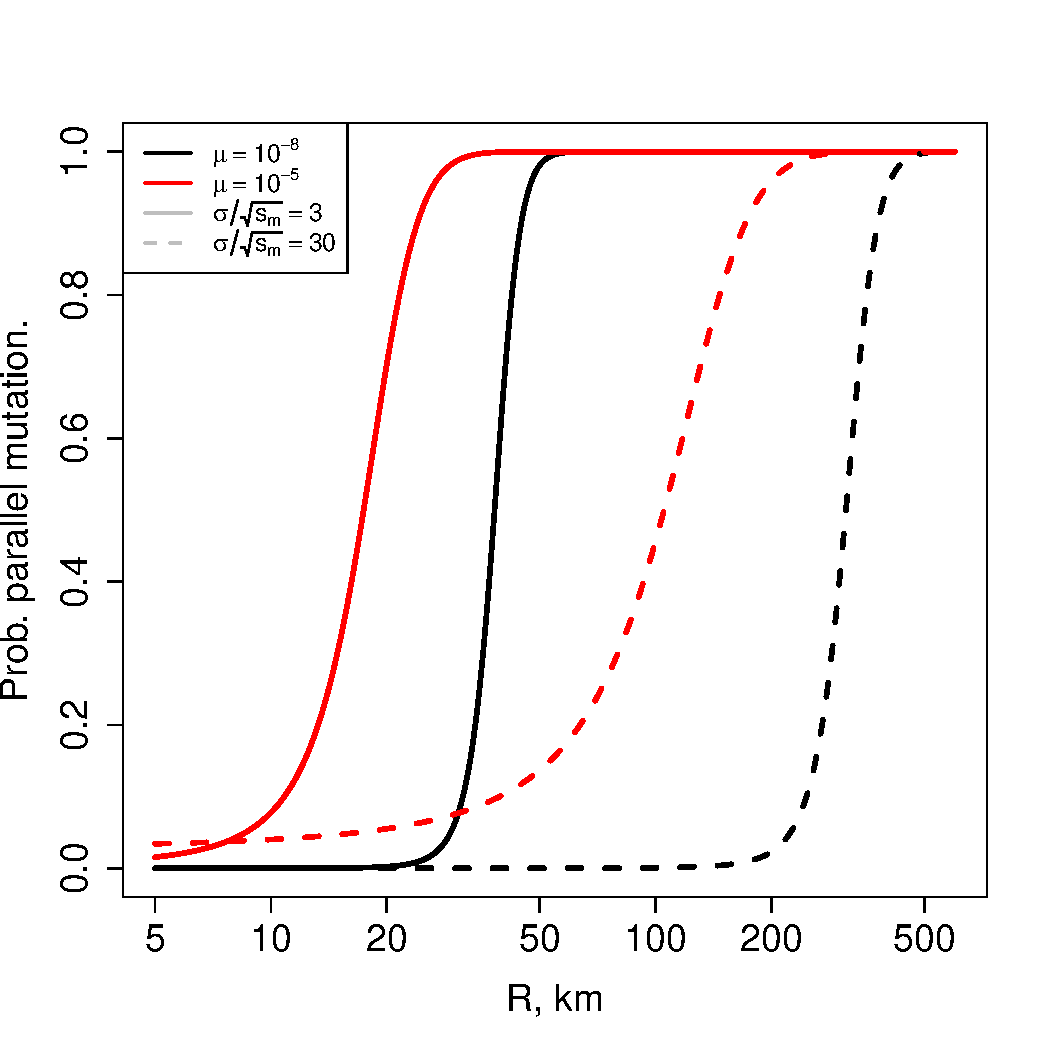
\includegraphics{Lava_flow_mice_prob_parallel}
  \end{center}
  \caption{
The probability of parallel mutation as a function of the distance
between environmental patches for two different cline widths
and two different mutation rates (using equation \eqref{eqn:parallel_prob}). 
The parameters were chosen to match the example of \textit{Chaetodipus intermedius};
see text.
  \label{fig:mice_prob_parallel}
  }
\end{figure}

The mutational target size $\mu$ for the trait is unclear. 
While the Pinacate dark haplotype differs from the light haplotype at three amino acid residues,
it is likely that not all of these changes are needed for a population to begin to adapt. 
Also there a number of genes besides MC1R at which adaptative changes affecting pigmentation 
have been identified in closely related species and more broadly across vertebrates \citep{Hoekstra:06}.
To span a range of plausible values, we use a low mutation rate of $\mu= 10^{-8}$, 
where the adaptive mutation has to occur at a single base pair; 
and a high mutation rate $\mu= 10^{-5}$, equivalent to the mutation
being able to arise at any of a thousand base pairs.  
Finally, we set $A=100\text{km}^2$ (roughly the size of the Pinacate patch).
Figure~\ref{fig:mice_prob_parallel} shows the dependance of the probability
of parallel mutation on the distance between lava flow patches using these parameters, 
showing that parallel mutation should become
likely over a scale of tens to a few hundred kilometers between patches. 

Given the large selection coefficient associated with the dark allele
on the dark substrate, we expect the initial haplotype associated with
either a new mutation or migrant allele to be large. 
We can use equation \eqref{eqn:haplotype_length} to calculate how long the founding
haplotype shared between populations is expected to be,
as shown in Figure~\ref{fig:mice_prob_parallel}. 
The initial length can be quite long between geographically close patches (tens of kilometers). 
However, for the wider cline width ($\sigma/\sqrt{s_m} = 30$km), 
adaptation by migration can still be likely for patches 100km apart, 
but the shared basis may be hard to detect, as the length of shared haplotype can be quite short. 

Furthermore, given the relatively small radius of the patches of dark substrate (often $<10$km),
we should expect the haplotype to be rapidly whittled down within
patches after establishment (equation \ref{eqn:rec_rate_within}). We
estimate that the effective recombination rate is at most only 50 \% lower
than the actual recombination rate.
Indeed, if we take the population density to be roughly $\rho \approx 10$ per hectare (M.~Nachman, personal communication),
and the variance in offspring number to be $\xi^2 = 3$ (mostly to get round numbers),
then the shared haplotype length within patches from equation \eqref{eqn:within_haplotype_length}
is only expected to be on the order of hundreds or thousands of bases
($10^{-3}$--$10^{-4}$cM).
This suggests that unless the migration has happened fairly recently
then it will be difficult to identify shared haplotypes
(how recently depends on the background level of LD in the population).


%%%%%%% %%%%%%% %%%%%%%
\section{Discussion} 
\label{ss:discussion}

This paper is an investigation into the basic question: 
What is the spatial resolution of convergent local adaptation?
In other words, 
over what spatial scale of environmental patchiness will evolution develop independent solutions to evolutionary problems?
The answer to this depends most strongly on $\sigma/\sqrt{s_m}$, 
the dispersal distance divided by the square root of the strength of selection
against the new allele between patches. It depends much more weakly on the
selective benefit within the patches or (perhaps suprisingly) the population density, 
although these two factors will determine the time-scale over which adaptation will occur. 
This is in contrast with models of panmictic populations \citep{softsweepsI} 
and geographically spread populations adapting to homogeneous selection pressures \citep{ralph2010parallel}, 
where the probability of multiple, independently arising adaptive alleles increases with the population size/density. 
However, in all of these models the dependence on the beneficial selection
coefficient is absent or weak, due to the fact that selection both
aids establishment of new alleles and the spread of existing
alleles. 

We have also shown that
while weaker selection against alleles will make sharing 
of adaptations between patches easier, 
it will also makes it harder to spot the sharing,
since the lucky alleles that manage to colonize new patches move slower,
and thus carry a shorter shared haplotype.
This issue is amplified by the fact that the length of haplotype
shared within patches decays over time, potentially making the
identification of shared adaptations to old selection pressures difficult.

In this work, we have tried to emphasize an intuitive, individual-centered understanding of the process,
determining, for instance, 
the speed at which successful migrants traverse regions where they are maladapted,
and the effective rate at which new families of migrant alleles appear
at long distances from a patch.
These quantities may be as useful for applied work
as more abstract ones such as the probability that adaptation occurs by migration versus new mutation.


\paragraph{Standing variation} 
We have tended to focus on relative rates of adaptation,
since we are thinking of applications in which we know that adaptation has occurred,
and the question is whether or not adaptations in distinct patches
have appeared indpendently or not.
However, especially if rates of adaptation by new mutation are very low,
any adaptation that does occur may have to make use of standing variation.
The unstructured case was studied by \citet{softsweepsI};
we study the continuous, spatial case in an upcoming paper.
If parallelism in local adaptation of the sort we study here is due to standing variation
rather than new mutation,
then the dynamics of adaptation should not depend strongly on migration patterns
(but note that the initial spatial distribution of standing variation may be).

\paragraph{Dominance}
We have mostly swept the issue of dominance under the rug
by dealing with essentially haploid models,
and appealing to the fact that the dynamics we study occur where the mutation is rare,
and hence mostly present only in heterozygotes. 
Our results should hold as a good approximation to dominant and partially dominant alleles
(with $s_m$ the selection against heterozygotes).
If, however, the mutation is recessive, then it is essentially neutral where rare,
and so would encounter much less resistance to spreading between patches.
This is counteracted, however, by the increased difficulty with which the mutation would establish
once arriving in a new patch. 
As such it is not clear what our intuition should be 
about the contribution of recessive alleles to adaptation via migration. 
Further work is needed to put empirical observations of local adaptation by recessive alleles 
in a theoretical context.

\paragraph{Long distance migration}
We have also ignored the possibility of very long distance migration,
instead focusing on local dispersal (and using a Gaussian model).
However, dispersal distributions can be very heavy tailed, 
with a small fraction of individuals moving very long distances indeed \citep{levin2003ecology,reynolds2009levy}.
In addition, over long time-scales, very rare chance events (mice sucked up in hurricanes and the like) 
could play a role in spreading migrant alleles if adaptation by other means is sufficiently unlikely.
Such tail events could greatly increase the probability of parallel adaptation above that predicted by our model. 
Furthermore, if adaptive alleles do move between distant patches via rare, long distance migration 
then they will be associated with a much longer shared haplotype than predicted by equation \eqref{eqn:haplotype_length}. 
As such, we view our results as a null model by which the contribution of long distribution migrants to adaptation could be empirically judged.   

\paragraph{Other patches geometries}
Here we have studied circular patches of habitat at long distances from each other,
while real habitat is can be much more complex
-- archipelagos of patches of varying sizes, or connected by long, skinny corridors, for instance.
The work of \citet{cantrell1991diffusive} comes closest to a general theory of balanced polymorphisms in such habitats,
and it is possible that our techniques could be applied in their much more general setting,
as both are based, fundamentally, on branching process approximations.



\paragraph{Concluding thoughts}
The falling cost of population genomic sequencing means that we will soon have the
opportunity to study the interplay of adaptation with geography and ecology 
across many populations within a species. 
Our work suggests that even quite geographically close populations 
may be forced to adapt convergently when migration is geographically limited. 
Thus, systems where populations have been repeatedly subject to 
strong local selection pressures may offer the opportunity 
to study highly replicated convergent adaptation within a similar
genetic background \citep{Stern:13}.  
Such empricial work will also strongly inform our understanding of how gene flow 
may work to keep ecologically similar populations evolving in concert \citep{sexton2013genetic}.
Our results suggest that adaptation to shared environments is
certainly no guarantee of a shared genetic basis to adaptation, 
suggesting that rapid adaptation to a shared environment could potentially drive
speciation under some scenerios \citep[in a manner similar to ][]{}. 

% discussion of applications. 

% discuss mixing of types; 
% Graph: from simulation showing local proportions in a single patch showing initial fixation of a single type and later mixing converging toward more than one type.  (and eventual loss of one?)

% unequal density: Lenormand, gene flow and limits of\dots


\bibliography{standing_patches_refs}

\appendix

%%%%%
\section{Numerical calculation of the probability of establishment}
\label{apx:establishment_sims}

To investigate the impact of the various approximations surrounding the mutational influx,
we calculated the probability of establishment for an spatial branching process moving across discrete demes.
The solution was obtained by iterating the multivariate generating function until convergence
(since the function which gives the probability of extinction as a function of location of the progenitor
is an attractive fixed point of the generating function; see \citet{jagers1975branching}).
These solutions are shown, and parameters described, in figure~\ref{fig:prob_estab_calcs}.

Here (and at other parameter choices) we see that the probability of establishment $p(x)$ goes to the equilibrium value
(approximately $p_e = 2s/\xi^2$) within the patch;
the transition is fairly symmetrical about the edge of the patch, even if the edge of the patch is not sharp.
This lends credence to our approximation that the integral of $p(x)$ over the entire range
is close to $p_e$ multiplied by the area of the patch.

\begin{figure}[ht!]
    \begin{center}
        % made in patchy-selection-plots.R
        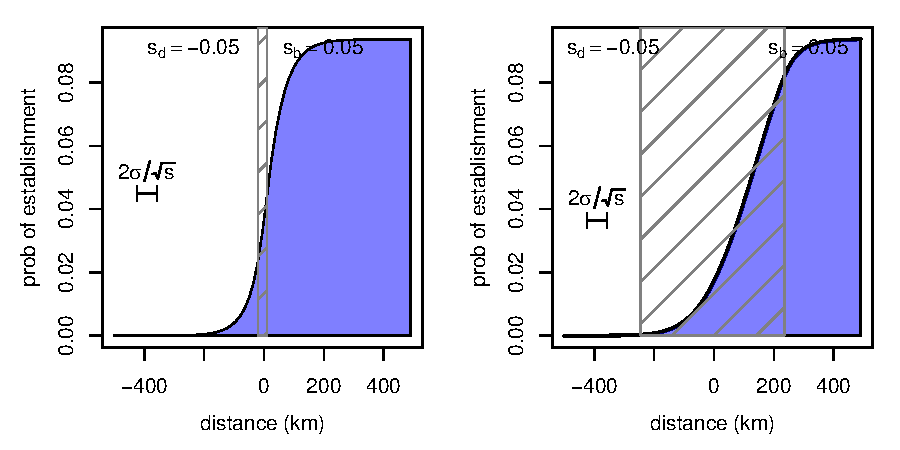
\includegraphics{prob-establishment}
    \end{center}
    \caption{The probability of establishment of a new mutant allele as a function of distance from the edge of the region where it is beneficial,
    in an abrupt transition (left) and a gradual transition (right).
    The allele is deleterious to the left and beneficial to the right (with selection coefficients $\mp 0.05$ respecively);
    and the selection coefficient interpolates linearly between these in the central hatched region.
    The number of offspring is Poisson.
    The underlying landscape has demes every 15km and a migration rate of 0.5 between neighboring demes;
    the probability was found by numerically solving the equation for the probability of establishment of a multi-type branching process.
    \label{fig:prob_estab_calcs}
    }
\end{figure}


%%%%%%%%%%%%
\section{The equilibrium frequency}
\label{apx:eqfreq}

For completeness, and clarity as to the scalings on the relevant parameters,
here we provide a derivation of the differential equations referred to above equation~\eqref{eqn:eqfreq},
and establish the asymptotics given in that equation.
One route to the ``equlibrium frequency'' of the allele outside the range where it is advantageous is as follows;
see \citet{slatkin1973geneflow} or \citet{barton1987establishment,pollak1966survival} for other arguments in this case, 
or \citet{etheridge2000introduction} and/or \citet{dawson1993measurevalued} for general theory used below.
Following is a description of a discrete model (which is nearly the one we simulate from).
Suppose that the population is composed of a finite number of small demes of equal size $N$ arranged in a regular grid,
and that selection (for or against) the allele is given by the function $s(x)$, with $x$ denoting the spatial location.
Each individual at location $x$ reproduces after a random lifetime,
dying, and then leaving behind in the same deme a random number of offspring with distribution given by $X$;
each offspring then migrates independently to a new location chosen randomly from the distribution given by $x+R$,
where she replaces a randomly chosen individual.
If $x+R$ is outside of the range, then she perishes.
Each individual's time until reproduction is exponentially distributed:
the reproduction rate is 1 if it carries the original allele, or with rate $1+s(x)$ if it carries the mutant allele.
Suppose that the number of offspring $X$ has mean $\mu$; the variance of $X$ will not enter into the formula.
Also suppose that the migration displacement $R$ has mean zero and variance $\sigma^2$;
if we are in more than one dimension, we mean that the components of the dispersal distance are uncorrelated
and each have variance $\sigma^2$.
We also assume that the distribution of $R$ makes the associated random walk irreducible and aperiodic.

Let $\Phi^N_t(x)$ be the proportion of mutant alleles present at location $x$ at time $t$,
and $\Phi_t(x)$ the process obtained by taking $N \to \infty$ (which we assume exists).
Denote by $\delta_x$ a single unit at location $x$, so that e.g.~$\Phi^N_t + \delta_x/N$
is the configuration after a mutant allele has been added to location $x$.
For $0\le \phi \le 1$, we also denote by $\bar X_\phi$ the random number of mutant alleles added if $X$ new offspring carrying mutant alleles
replace randomly chosen individuals in a deme where the mutant allele is at frequncy $\phi$ (i.e.~hypergeometric with parameters $(X,\phi)$);
similarly, $\widetilde X_\phi$ is the number lost if the new offspring do not carry the allele (i.e.~hypergeometric with parameters $(X,1-\phi)$).
(We like to think of $\Phi^N_t$ as a measure, but it does not hurt to think of $\Phi^N$ as a vector;
we aren't providing the rigorous justification here.)
Then we know that for any sufficiently nice function $f(\Phi)$ that
\begin{align} \label{eqn:discrete_generator}
  \begin{split} \frac{\partial}{\partial t} \E\left[ f(\Phi^N_t) \right] 
  &= N \sum_x \left\{ \E\left[ (1+s(x+R)) \Phi^N_t(x+R) \left( f\left(\Phi^N_t + \frac{\bar X_{\Phi_t(x+R)}}{N}\delta_{x}\right) - f(\Phi^N_t) \right) \right] \right. \\
     & \qquad  \qquad \left. {} + \E\left[ \left(1-\Phi^N_t(x+R)\right) \left( f\left(\Phi^N_t - \frac{\widetilde X_{\Phi_t(x+R)}}{N}\delta_{x}\right) - f(\Phi^N_t) \right) \right] \right\}  \end{split} \\
     &= \mu \sum_x \E\left[ \left(\partial_{\phi(x)} f(\Phi_t) \right) \left\{ \Phi_t(x+R) - \Phi_t(x) + s(x+R) \Phi_t(x+R) (1-\Phi_t(x)) \right\} \right] + O\left(\frac{1}{N}\right).
\end{align}
In the final expectation, $R$ and $\Phi$ are independent.
This follows by taking first-order terms in $1/N$ in the Taylor series for $f$, 
and the fact that $\E[\bar X_\phi] = \phi \mu$ and $\E[\widetilde X_\phi] = (1-\phi)\mu$.
We can see two things from this:
First, since this is a first-order differential operator, the limiting stochastic process $\Phi$
is in fact deterministic (check by applying to $f(\Phi) = \Phi(x)^2$ to find the variance).
Second, if we want to rescale space as well to get the usual differential equation, 
we need to choose $\var[R]=\sigma^2$ and $s(x)$ to be of the same, small, order; 
this is another way of seeing that $\sigma/\sqrt{s}$ is the relevant length scale \citep[as noted by][]{slatkin1973geneflow}.
More concretely, suppose that the grid size is $\epsilon \to 0$, 
that $\var[R] = (\sigma \epsilon)^2$, and that $s(x)/\epsilon \to \gamma(x)$,
and suppose that $\Phi_t(x)$ is deterministic (and sufficiently differentiable) and let $\xi(t,x) = \Phi_{t/\epsilon}(x)$;
then the previous equation with $f(\Phi) = \Phi(x)$ converges to the familiar form:
\begin{align}
  \label{eqn:derived_fkpp}
  \partial_t \xi(t,x) = \mu \left( \frac{\sigma^2}{2} \sum_{k=1}^d \partial_{x_k}^2 \xi(t,x) + \gamma(x) \xi(t,x) (1-\xi(t,x)) \right) .
\end{align}
Here we have taken first the population size $N \to \infty$ and then the grid size $\epsilon \to 0$;
we could alternatively take both limits together, but not if $\epsilon$ goes to zero too much faster than $N$ grows.
One reason for this is that at finite $N$,
the process $\Phi_t$ is an irreducible, aperiodic finite-state Markov chain with absorbing states at 0 and 1;
therefore, the inevitable outcome is extinction of one type or another,
which is not the regime we want to study.

In one dimension, we are done (see section~\ref{apx:elliptic_integrals});
in higher dimensions, we are more interested in the mean frequency at a given distance $r$ from a patch.
If we take a radially symmetric patch centered at the origin (so $\gamma$ only depends on $r$), 
and let $\xi(t,r)$ denote the mean occupation frequency at distance $r$,
then the polar form of the Laplacian in $d$ dimensions gives us that \eqref{eqn:derived_fkpp} is
\begin{align}
  \label{eqn:radial_fkpp}
  \partial_t \xi(t,r) = \mu \left( \frac{\sigma^2}{2} \partial_{r}^2 \xi(t,r) + \sigma^2\frac{d-1}{2r} \partial_r \xi(t,r) + \gamma(r) \xi(t,r) (1-\xi(t,r)) \right) .
\end{align}


%%%%%%%%%%%
\subsection{Asymptotic solution for the equilibrium frequency} 
\label{apx:asymptotics}

If $q(r)$ is a radially symmetric equilibrium frequency and $\xi(t,x)=q(|x|)$,
then $\partial_t \xi(t,x) = 0$.
So, using \eqref{eqn:radial_fkpp}, a radially symmetric solution 
with $\gamma(r) = -s < 0$ for all $r>r_0$ 
solves, for $r_0 < r < \infty$,
\begin{align}
    \partial_r^2 q(r) + \frac{d-1}{r} \partial_r q(r) - \frac{2s}{\sigma^2} q(r) (1-q(r)) = 0 \\
    \lim_{r \to \infty} q(r) = \lim_{r \to \infty} \partial_r q(r) = 0 \qquad 
    0 < q(r) < 1 
\end{align}
Since $q(r) \to 0$ as $r \to \infty$, so $q(r) (1-q(r)) \approx q(r)$,
it can be shown 
% theory in \citet{wasow1965asymptotic} implies 
that the true equilibrium frequency $q$ is close, for large $r$, to the solution to
\begin{align}
    \partial_r^2 u(r) + \frac{d-1}{r} \partial_r u(r) - \frac{2s}{\sigma^2} u(r) = 0  \label{eqn:bessel} \\
    \lim_{r \to \infty} u(r) = \lim_{r \to \infty} \partial_r u(r) = 0 \qquad  .
\end{align}
This has general solution given by a modified Bessel function:
using \citet{gradshteyn2007table} 8.494.9,
the general solution is
\begin{align}
    u(r) = C' (r-r_0)^{(2-d)/2} K_{(2-d)/2} \left( (r-r_0) \sqrt{2s}/\sigma \right) ,
\end{align}
where $C'$ and $r_0$ are chosen to match boundary conditions.
Asymptotics of Bessel functions \citep[][8.451.6]{gradshteyn2007table} then imply that
\begin{align}
    q(r) \approx C r^{(1-d)/2} \exp \left( -r \sqrt{2s}/\sigma \right) + O(1/r),
\end{align}
where $C$ is a different constant.



%%%%%%%
\subsection{The exact solution to the equilibrium frequency}
\label{apx:elliptic_integrals}


Here we describe how to solve \eqref{eqn:derived_fkpp} in one dimension,
i.e.\ the Fisher-KPP equation with varying selection.
Let $p(t,x)$ be the proportion of the allele under spatially varying selection $s(x)$ in one dimension,
so that 
\[
\partial_t p(t,x) = \frac{\mu}{2} \sigma^2 \partial_x^2 p(t,x) + \mu s(x) p(t,x) (1-p(t,x)) .
\]
The stable distribution $\phi(x) = \lim_{t\to\infty} p(t,x)$ then solves
\begin{align} \label{eqn:definingphi}
    \partial_x^2 \phi(x) = - 2 s(x) \phi(x) (1-\phi(x)) /\sigma^2,
\end{align}
with appropriate boundary conditions.
First rescale space by $\sigma/\sqrt{2}$ so the $\sigma^2/2$ term dissappears.
If we now assume that $s(x)$ is piecewise constant,
$s(x) = s_i$ for $x \in [x_i,x_{i+1})$, with $x_0=-\infty$ and $x_{n+2}=\infty$,
then the equation is integrable: if we multiply through by $2\partial_x \phi(x)$ and integrate, then we get that
\begin{align} \label{eqn:conservation}
    ( \partial_x \phi(x) )^2  &= - \int^{x} 2 s(x) \phi(x) (1-\phi(x)) \partial_x \phi(x) dx \\
        &= - s_i \phi(x)^2 \left( 1 - \frac{2}{3} \phi(x) \right) - K_i \quad \mbox{for } x \in [x_i,x_{i+1}) ,
\end{align}
if we define
\begin{align} 
  K_i = - s_i \phi(x_i)^2 \left( 1 - \frac{2}{3} \phi(x_i) \right) - ( \partial_x \phi(x_i) )^2  .
\end{align}
For ease of reference, we define
\[
        V_i(\phi) = s_i \phi^2 \left( 1 - \frac{2}{3} \phi \right) + K_i .
\]
Note that $V_i'(0)=V_i'(1)=0$, that $V_i(0)=K_i$ and $V_i(1) = K_i+s_i/3$.  
We will always have that $V(\phi) \le 0$.
(We have then that $\partial_x^2 \phi = - \partial_\phi V(\phi)$, the equation of motion of a particle in potential $V$.
Also note that this implies ``conservation of energy'', i.e.\ $( \partial_x \phi(x) )^2 + V(\phi(x))$ is constant.)
Rearranging, we get that $dx = d\phi / \sqrt{-V(\phi)}$, so where $\phi(x)$ is monotone, the inverse is
\[
    x(\phi) = x(\phi^*) \pm \int_{\phi^*}^\phi \frac{ d\psi }{ \sqrt{ -V(\psi) } } .
\]
For each $i$ then define the elliptic function
\begin{align}  \label{eqn:elliptic_function}
    F_i(\phi) = \int_{\phi_i^*}^\phi \frac{ d\psi }{ \sqrt{ -V_i(\psi) } } ,
\end{align}
where take the positive branch of the square root, and $\phi_i^*$ will be chosen later.
Then we have that
$x(\phi) - x(\phi_0) = \pm( F(\phi) - F(\phi_0))$,
or for an appropriate $x_0$,
\[
    \phi(x) = F^{-1}\left( F(\phi(x_0)) \pm (x - x_0) \right).
\]

We clearly want $\lim_{x \to \infty} \partial_x \phi(\pm x) = 0$, 
and $\lim_{x \to \infty} \phi(\pm x)$ to be zero or one depending on the sign of $s_0$ and $s_{n+1}$.
Since $(\partial_x \phi(x))^2 = -V(x)$, this implies that if $s_0<0$, then $K_0 = 0$,
while if $s_0>0$ then $K_0 = s_0/6$; and likewise for $K_{n+1}$.

We also require that $\phi(x)$ and $\phi'(x)$ are continuous.
Continuity of $\phi'(x)$ is equivalent to $V_i(x_{i+1}) = V_{i+1}(x_{i+1})$,
which we can rearrange to find an equation for $K_{i+1}$ in terms of $K_i$ and $\phi(x_{i+1})$:
\[
    K_{i+1} - K_i = (s_i - s_{i+1}) \phi(x_{i+1})^2 (1-2\phi(x_{i+1})/3) .
\]
What about the frequency at the points the selection changes, $\phi(x_i)$?  
Well, if $\phi(x)$ is monotone on $[x_i,x_{i+1})$ then we can without loss of generality take $\phi_i^*=0$ or $1$ depending on the sign of $s_i$.
Otherwise, let $\phi_i^*$ be the (unique) root of $V_i$ in $[x_i,x_{i+1})$, so $V_i(\phi_i^*)=0$.
In this case, $\phi_i^*$ is the maximum or minimum of $\phi$ in the interval:
if $s>0$, then $\phi_i = \max\{ \phi(x) : x \in [x_i,x_{i+1})\}$. 
Recall we defined $F_i$ using $\phi_i^*$; now using the fact that $\phi$ is monotone with the opposite sign on either side of $\phi_i^*$,
$x_{i+1} - x_i = F_i(\phi(x_{i+1})) - F_i(\phi_i^*) + F_i(\phi(x_{i})) - F_i(\phi_i^*)$,
and that $F(\phi_i^*) = 0$,
we know that the length of the $i$th stretch is
\[
    x_{i+1} - x_i = \pm \left( F_i(\phi(x_i)) + F_i(\phi(x_{i+1})) \right).
\]
Note that all the $\pm{}$'s are easily relatable to the signs of $s_i$.
If we knew $\phi(x_1)$ and $\phi'(x_1)$, then we'd be able to solve the equations for $\phi(x_i)$ and $K_i$ recursively upwards.
In some cases, such as \citet{slatkin1973geneflow}, we can infer $\phi(0)$ and $\partial_x \phi(0)$ by spatial symmetry.
In other cases, we are only given $\phi(-\infty)$ and $\phi(\infty)$, and have to work inwards from the ends.


\subsection{Doing the integrals}
\label{apx:some_integrals}

An important ingredient in the above method is the integral \eqref{eqn:elliptic_function},
to which a method for solving the Korteweg-de Vries equation can be applied \citep{NEQwiki}.
Recall that $V_i(\phi) =  s_i \phi^2(1-2\phi/3) + K_i$, with $K_i = V_i(0)$ chosen to match $V$ at the boundaries;
since we're just working within an interval with $s$ constant, we can rescale space by $\sqrt{2 s_i}/\sigma$,
so that $s$ and $\sigma$ drop from the equation.
We then want to integrate
\[
    \int \frac{ d\phi }{ \sqrt{-V(\phi)} } = 
         \int \frac{ d\phi }{ \sqrt{ \phi^2 (1-2\phi/3) + K } } ,
\]
over a domain where $V$ is always negative.
Let $\phi^2(1-2\phi/3)+K = (\alpha-\phi)(\phi-\beta)(\phi-\gamma)$,
and change variables first to $y^2=(\alpha-\phi)$, 
and then to $x = y/\sqrt{\alpha-\beta}$, so that
\begin{align*}
    \frac{ d\phi }{ \sqrt{ \phi^2 (1-2\phi/3) + K } } 
        = \frac{ - 2 dy }{ \sqrt{ (\alpha-\beta-y^2) (\alpha-\gamma-y^2) } } \\
        = \frac{ - 2 dx }{ \sqrt{\alpha-\gamma} \sqrt{ (1-x^2) (1-S^2 x^2) } } ,
\end{align*}
with $S^2 = (\alpha-\beta)/(\alpha-\gamma)$.
Now Jacobi's incomplete elliptic integral of the first kind is defined by
\[
    F(x;k) = \int_0^x \frac{dt}{\sqrt{ (1-t^2)(1-k^2t^2) }} ,
\]
and the Jacobian elliptic function $\sn(x;k)$ is the inverse: $F(\sn(x;k);k) = x$.
As $k \to 0$, $\sn(x;k) \to \sin(x)$, while as $k \to 1$, $\sn(x;k) \to \sinh(x)$.

% Presumably, this gets the same answer as \citep{slatkin1973geneflow}, who finds that in the solvable cases,
% for $x$ in the last interval (which ends in $\infty$), that
% \begin{align*}
%     \phi(x) &= \frac{3}{2}\left( 1 - \tanh^2 ( x \sqrt{2s} / 2 \sigma + C ) \right) \\
%         &\simeq C' \exp\left( - \frac{ x \sqrt{2s} }{ \sigma } \right) .
% \end{align*}



%%%%%%%%% %%%%%%%%%%%%%%
\section{Hitting and occupation}
\label{apx:hitting_occupation}

Consider a single migrant family $Z$ beginning at $x$,
and write $S$ for the new patch, which has area $A$ and is centered at $y$.
Let $B_t$ be a Brownian motion with variance $\sigma^2$, 
and $\tau_\dagger$ an independent Exponential($s_m$) time.
The mean occupation time of $Z$ spent in a region $S$ is,
since the marginal distribution of a single lineage is Brownian,
\begin{align}
    u(x,S) &= \E[\int_0^\infty Z_t(S) dt ] \\
           &= \int_0^\infty \E[Z_t] p_t(x,S) dt \\
        &= \int_0^\infty e^{-s_m t} p_t(x,S) dt \\
        &= \int_0^\infty \P^x\{ \tau_\dagger > t \; \& \; B_t \in S \} dt \\
        &= \E\left[ \int_0^{\tau_\dagger} \one_S(B_t) dt \right]  .
\end{align}
If we define
$\tau_S$ to be the hitting time of $S$ by the Brownian motion $B$,
and $\mu_S(x)$ to be the hitting distribution of $\partial S$ by $B_{\min(t,\tau_\dagger)}$,
by the strong Markov property this is equal to
\begin{align}
    u(x,S) % &= \E^x[ \int_0^{\tau_\dagger} \one_S(B_t) dt ] \\
           &= \P^x\{ \tau_S < \tau_\dagger \}  \E^{\mu_S(x)}\left[ \int_0^{\tau_\dagger} \one_S(B_t) dt \right] ,
\end{align}
provided $S$ is not pathological.
If $S$ is circular with area $A$, the latter expectation will not depend on $x$;
call this $g(A)$.

Now consider the chance that $Z$ ever hits the new patch, which we call $h(x,S)$.
(In the main body, this was $h_A(x,y)$, here modified to parallel $u(x,S)$.)
If we make the approximation that $Z$ hits the new patch only if the trunk of $Z$ does,
and recall that $1-k_e(t)$ is the chance that $Z$ survives for $t$ generations,
then this is equal to
\begin{align}
    h(x,S) &= \int_0^\infty (1-k_e(t)) \P\{ \tau_S \in dt \} \\
           &= \int_0^\infty e^{s_m t} (1-k_e(t)) e^{- s_m t } \P\{ \tau_S < t \} dt \\
    &=\int_0^\infty e^{s_m t} (1-k_e(t)) \P\{ \tau_S < t < \tau_\dagger \} dt \\
    &\approx \frac{1}{\E[K]} \int_0^\infty \P\{ \tau_S < t < \tau_\dagger \} dt \\
    &= \frac{1}{\E[K]} \P^x[ \tau_S < \tau_\dagger ] .
\end{align}
Therefore, we have that
\begin{align}
    h(x,S) \E[K] 
    \approx \P^x[ \tau_S < \tau_\dagger ] 
    = u(x,S) / g(A) .
\end{align}

If we let $q(S) = \int_S q(y) dy$ be the total equilibrium occupation of $S$,
then by equation~\eqref{eqn:migrate_integral},
\begin{align}
    q(S)  &= \int_{\partial B(r_0)} \gamma(x) u(x,S) dx  \\
          &\approx g(A) \E[K] \int_{\partial B(r_0)} \gamma(x) h(x,S) dx \\
          &= \frac{ g(A) \E[K] }{ \rho f(A) } \migrate(y) .
\end{align}
The function $g(A)$ is the expected amount of time that a Brownian motion begun on the edge of a disk of area $A$
is expected to spend inside the disk before $\tau_\dagger$.
This is integral of the Green function for the Bessel process of the appropriate order, 
so using \citet{borodin2002handbook}, % (Appendix 1),
and letting $w$ be the width of the patch,
in $d=1$,
\begin{align}
    g(A) % &= \E^w[ \int_0^\tau \one_A(B_t) dt ] 
    % &= \int_0^{2w} G_{s_m}(0,y) dy \\
  &= \int_0^{2w} \frac{ e^{- y \sqrt{2s_m} }}{\sqrt{2s_m}} dy \\
  &= (1-e^{-2w\sqrt{2s_m}})/(2s_m)
\end{align}
and in $d=2$, by \citet{gradshteyn2007table} 5.56.2,
\begin{align}
    g(A) % &= \E^w[ \int_0^\tau \one_A(B_t) dt ] 
    % &= \int_0^{2w} G_{s_m}(0,y) dy \\
  &= \int_0^{2w} 2 y K_0(y \sqrt{2s_m}) dy \\
  &= \frac{1}{s_m}\int_0^{2w\sqrt{2s_m}} y K_0(y) dy \\
  &= \frac{1}{2s_m}\left(1- 2w\sqrt{2s_m} K_1(2w\sqrt{2s_m}) \right)  .
\end{align}
In either case, $g(A) \approx 1/(2s_m)$, which is the approximation we use in the main text.




%%%%%%% %%%%%%%%%%%%
\subsection{The outflux of families}
\label{apx:outflux}

It is of interest to have an expression for the ``outflux of families'',
$\gamma(r_0)$, 
defined to be the mean proportion of $B$ alleles at distance $r_0$
whose lineage traces back to the original patch without venturing further away than $r_0$.
By expression \eqref{eqn:occupation_integral},
\[
    \gamma(r_0) = \frac{q(y)}{\int_{B(r_0)} u(x,y) dx}
\]
for any $y$.  
Take $y=(r,0)$.
Note that after scaling by $\sqrt{2s_m}/\sigma$,
\begin{align}
    \frac{ u(x,y) }{ q(y) } &\simeq C' \frac{ \|y-x\|^{-(d-1)/2} e^{-\|y-x\|} }{ \|y\|^{-(d-1)/2} e^{-\|y\|} } \\
        &= C' \| \hat x - x/r \|^{-(d-1)/2} e^{-r (\|\hat x - x/r\| - 1)} .
\end{align}
Now let $x = (r_0 \cos \theta, r_0 \sin \theta)$,
so that the expression in the exponent is to, first order in $1/r$,
\begin{align}
    r (\|\hat x - x/r\| - 1) &= r \left( \sqrt{ \left( 1 - \frac{r_0}{r} \cos \theta \right)^2 + \frac{r_0^2}{r^2} \sin^2 \theta } - 1 \right ) \\
            &= - 2 r_0 \cos \theta + O(1/r) .
\end{align}
This implies that, still with $r$, $r_0$, and $\theta$ defined as above,
\begin{align}
    \frac{u(x,y)}{q(y)} \longrightarrow_{r \to \infty} C' e^{-2 r_0 \cos \theta} .
\end{align}
In one dimension we are done.
In two dimensions,
by bounded convergence and \citet{gradshteyn2007table} (3.339),
\begin{align}
  \int_{B(r_0)} \frac{u(x,y)}{q(y)} dx &\to \gamma(r_0) \quad \text{as } y \to \infty\\
            &= C' \int_0^{2 \pi} e^{-2 r_0 \cos \theta} d\theta \\
                         &= 2 \pi C' I_0(-2r_0),
\end{align}
where $I_0$ is a modified Bessel function of order zero of the first kind.
The effect of the scaling is to express $r_0$ in natural units, i.e.\ changing the result to $2 \pi C' I_0( - 2 \sqrt{2s_m} r_0 / \sigma ) $.

\section{UNUSED AFTER HERE?}

%%%%%%%%%
\section{Simulations of a patchy environment}
\label{apx:patchy_sims}

Describe sims.

Argue that $C=0.5$ is a reasonable number.

\begin{figure}[ht!]
    \begin{center}
        % made in patchy-sim-writeup-plots.R
        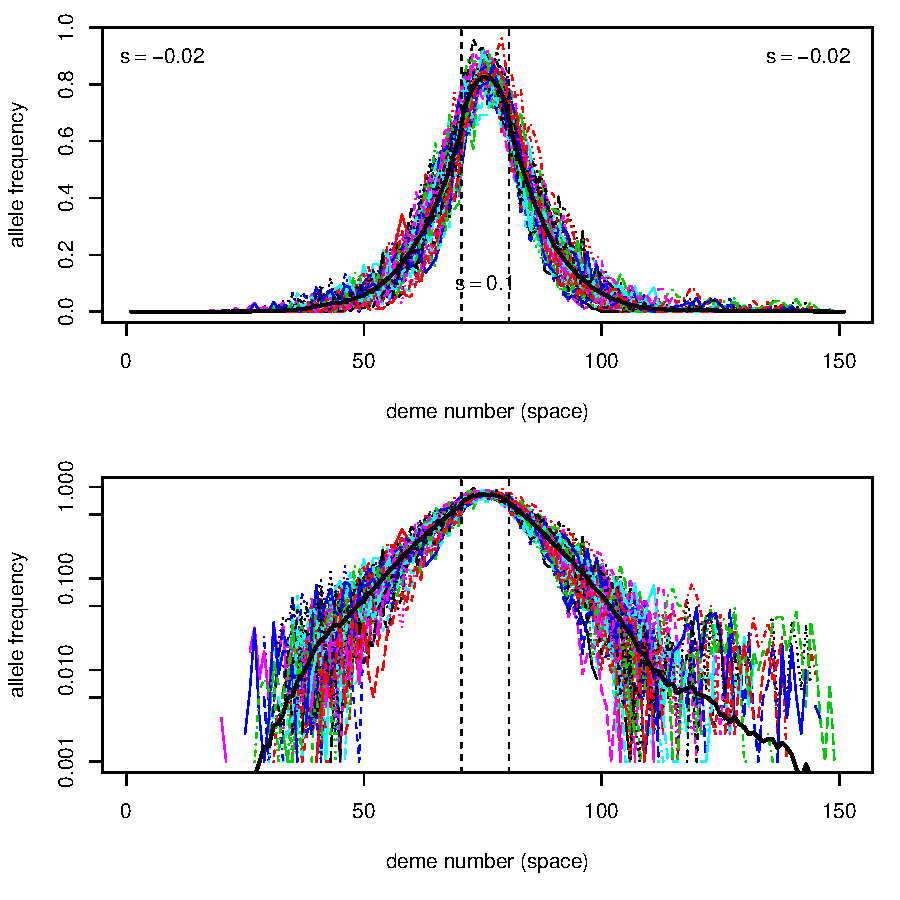
\includegraphics{example-equilibrium}
    \end{center}
    \label{fig:example_equil}
    \caption{
    Snapshots of a simulation of allelic frequency dynamics around a patch where the allele is beneficial:
    the focal allele is benefical in the middle region and deleterious outside.
    The dynamics were simulated for 10000 generations across demes with 1000 individuals in each
    and random dispersal to nearby demes with a mean dispersal distance of $\sigma \approx 2$ demes.
    Colored lines show allele frequencies across space in 50 uniformly spaced generations;
    the solid line shows the mean across all generations.
    Below is the same plot, except on a log scale.
    }
\end{figure}

%%%%%%%%%%%
\section{Patchy selection} 
\label{ss:discretedemes}

We have been working in a continuous model of geographic space; 
in this section we move to a discrete model of isolated populations exchanging rare migrants,
but in section \ref{ss:patchyspace} discuss how a model with {\em patchy} selection can be approximated by such a discrete model.

Suppose now that we have a set of $L$ discrete populations of individuals that may reproduce or migrate,
and that migration and mutation are rare, so that the waiting times until either event is approximately exponential.
Suppose that for each pair of populations, labeled $i$ and $j$, the mean number of migrants that travel from $i$ to $j$ per generation
is $M_{ij}$ and that the mean number of new mutations appearing in population $i$ per generation is $\mu_i$.

{\tt Include cartoon here.}

If we suppose that fixation occurs on a faster time scale than mutation or migration,
so that it is very unlikely that two different migrants or mutants begin to fix locally in the same population,
then we can treat the process of extinction or local fixation as instantaneous 
(a limit previous studied by \cite{Slatkin:81}).
In this limit we may also ignore swamping effects of inmigration of nonmutant alleles.

In this case, we have the following picture.
The population at first starts out with no selected alleles. 
At some later time point suppose that there are $T$ different alleles present in the population, 
that the $k^\mathrm{th}$ allele is occupying demes $\{i^k_1, \ldots, i^k_{n_k}\}$, for $1\le k \le T$.
Let $I$ denote the set of all adapted demes, 
and let $J = \{j_1, \ldots, j_\ell\}$ denote the demes that have not yet adapted, with $\ell = L - \sum_k n_k$.
Then we are assuming that two types of event can happen which could change the state:
either at rate $\mu_j p_f$, an unadapted deme $j$ produces a new mutant, which fixes in this deme;
or at rate $M_{ij} p_f$, an adapted deme $i$ sends a migrant to unadapted deme $j$, which fixes in that deme.
Therefore, under these assumptions, the probability of fixation $p_f$ (and hence the selection coefficient)
only enter as a time scaling: for instance,
if we define $R = \sum_{j \in J} \left( \mu_j + \sum_{i \in I} M_{ij} \right)$,
then the total rate of such events is $p_f R$.
The probability that the next event results in, say, adaptation of deme $j$
is 
\[
 \left( \mu_j + \sum_{i \in I} M_{ij} \right) / R,
\]
and the probability that deme $j$ adapts through migration from deme $i$, given that deme $j$ is the next to adapt, is
$M_ij / R$,
while the probability that it adapts through a new mutation is $\mu_j / R$.

The main point here is that the final pattern,
and hence the likely extent of parallel adaptation,
is independent of the strength of selection.
This is in contrast to the continuous case, however, this observation is dependent on the assumption of weak migration
and fails to hold if different migrant lineages interact.
This can be viewed as a continuous-time Markov process XXX.
Explicit solutions are not available in the general case,
but if we specialize to a completely symmetric model (i.e.\ the ``island'' model),
then the mathematical picture is a pretty one.

\subsection{Symmetric patches}

Indeed, suppose that migration and mutation are symmetric: $M_{ij}=m$ and $\mu_j = \mu$ for all $j$ and $i\neq j$.
Suppose at some time the $k^\mathrm{th}$ allele is occupying $n_k$ demes, 
with $n = \sum_k n_k < L$.
Then at rate $(L-n) N \mu p_f + n (L-n) N m p_f$,
either a migration or mutation event happens.
With probability $\mu/(\mu + n m)$, it is a mutation,
and a new deme is randomly chosen and assigned a new allele.
With probability $n_k m / (\mu + n m)$,
the $k^\mathrm{th}$ type sends a successful migrant to a randomly chosen new island,
which is assigned the $k^\mathrm{th}$ allele.

This process is a continuous-time version of the ``Chinese restaurant process''
described in \citet{aldous1985exchangeability} and \citet{pitman1995partitions},
and so the final partition of types across demes has the Ewens sampling distribution with parameter $\mu/m$.
Again note that the selection coefficient, which is implicit in the probability $p_f$,
does not enter into the final distribution.

Now we can compute most properties we might want about the process.
For instance, the expected number of distinct mutational origins is
\begin{equation}
    \E\left[ \mbox{ \# of independent mutations } \right] = 
            1 + \frac{\mu}{m} \sum_{k=2}^L \frac{1}{k+(\mu/m)}. \label{discrete_expected}
\end{equation}
The probability that there is only a single successful mutation is
\begin{equation}
\P \left\{ \mbox{only one mutational origin} \right\} = 
            \prod_{k=1}^{L-1} \frac{ k }{ k+(\mu/m)} .
\end{equation}
More generally, suppose we sample a single deme, and are interested in the total number of demes $S$
(including the sampled one) that share the same fixed mutation as our sampled deme.
Then $S$ has distribution
\begin{equation} \label{eqn:Sdistrn}
\P\{ S=s \} = \frac{ (s-1)! (\mu/m)^{L-s} }{ \prod_{k=1}^{L-1} (k+(\mu/m)) } .
\end{equation}
Furthermore, if $L$ is large, then $S/L$ has probability density approximately
\begin{equation} \label{eqn:betadistrn}
   (\mu/m) (1-x)^{(\mu/m)-1}
\end{equation}
namely, is a $\mathrm{Beta}((\mu/m), 1)$ distribution--- see \cite{donnelly1989continuity} and \cite{perman1992sizebiased}.

% In Figure \ref{fig:discbyratio} we plot mean number of types and size (number of demes occupied) of a sampled type,
% for a model with 20 interconnected demes, across different parameter values.  
% This indicates that we need the population-scaled mutation and migration rates to be within a factor of about 100 of each other for parallel adaptation to leave an interesting pattern. If migration is faster, then a single type is likely to take over, while if migration is weaker, each deme is likely to come up with its own type.

The high connectedness of the discrete deme island model means that the expected number of distinct alleles, (Equation \eqref{discrete_expected}), 
grows with the $\log$ of the number of demes. This strongly contrasts with the continuous spatial model where the local nature of dispersal means that doubling the species range will double the number of mutations expected. 
Furthermore, while in the continuous model the areas occupied by distinct mutations are similar in area, in this strong-selection discrete island model, 
only a few types tend to dominate even as the number of demes (and thus, distinct types) grows large (see Equations \eqref{eqn:Sdistrn} and \eqref{eqn:betadistrn}).

A more general model would allow migration only along edges of some graph connecting the demes.
In the low migration limit such a model still produces a partition distribution independent of the selection coefficient,
but it does not in general have the Ewens distribution.
Another extension would be to include the time alleles need to achieve an intermediate frequency,
along the lines of \citet{Navarro:03}, which would reintroduce dependence on the selection coefficient.

\texttt{XXX omit this? XXX}
We have treated the time during which the selected allele is at intermediate frequency in a deme (about $\log(\sigma^2 \rho)/s_p$ generations) as negligible, 
which ignores migration events that occur while the mutation is spreading through the population. 
we now sketch of a more realistic approximation.
For each occupied--unoccupied pair of demes, if the number of mutant alleles in the occupied deme is $n(t)>0$,
then at time $t$, migrants from the occupied deme pass the selected allele to the unoccupied deme at rate $2 n(t) m p_f(s_p)$,
while newly arisen mutants arise and fix in the unoccupied deme at constant rate $2 N \mu p_f(s_p)$.
The selected type should grow approximately as $n(t)=\exp(s(t-t_0))$.
Of course, to follow this model through, we will have to account for multiple types within a single deme and other complications,
but we can at least make a few observations.
One is that the final distribution of types is no longer independent of $s_p$, which enters through the dynamics $n(t)$.
However, it is clear that increasing the selection coefficient $s$ will decrease the number of types (independent mutational origins),
while on the other hand, increasing the deme size $N$ will increase the number of types,
and that the case presented above is at the extreme (see also \cite{Navarro:03} for deterministic approximations). 



\end{document} 

\section{Temporary work: hitting probs}

Now consider the probability that a migrant family from $x$ will ever establish in the new patch,
which we assume has relatively small area $A$ and is centered at position $y$.
The probability that this family reaches $A$ by time $t$ is $(1-k_e(t))$
multiplied by the probability that the family reaches the patch, given survival.
If $t$ is large then the previous section argues that $(1-k_e(t)) \approx e^{-s_m t}/\E[K]$,
and the probability of reaching the patch by $t$ approximately the chance that a Brownian path
will have hit the patch by then.
If $w = A^{1/d}$ is the width of the patch, then 
this is the chance that a $d$-dimensional Bessel process begun at $\|y-x\|$ hits $w$ by time $t$.
Let $\tau_w$ be the hitting time of $w$,
so, integrating by parts, and using Borodin \& Salminen (2.2.0.1 and 4.2.0.1)
\begin{align}
    \int_0^\infty (1-k_e(t)) \P^x\{ \tau_w \le t \} dt  
    &\approx \int_0^\infty e^{-s_m t} \P^x\{ \tau_w \le t \} dt  / \E[K] \\
    &= \frac{1}{s_m \E[K]} \int_0^\infty e^{-s_m t} \P^x\{ \tau_w \in dt \} \\
    &= \frac{1}{s_m \E[K]} \E^x[e^{-s_m \tau_w}] \\
    &= 
    \frac{1}{s_m \E[K]} \times
    \begin{cases}
        e^{-(x-w) \sqrt{2s_m}} \qquad & d=1 \\
        \frac{ K_0(x\sqrt{2s_m}) }{ K_0(w\sqrt{2s_m}) } \qquad & d=2 
    \end{cases}
\end{align}
Note that the $d=2$ case
\begin{align}
    \frac{ K_0(x\sqrt{2s_m}) }{ K_0(w\sqrt{2s_m}) } = \sqrt{\frac{w}{x}} e^{-(x-w)\sqrt{2s_m}} ( 1 + O(1/w) ).
\end{align}


\section{Notes: for intro/discussion}

- leimu2008metaanalysis: local adaptation not ubiquitous but common; mostly in large population sizes.
- robertson1960theory: dependence of the degree of adaptation on Ne 
- lots of local adaptation stuff on plants and conservation genetics; ties into plasticity and range limits.
- but also: Neurospora (ellison2011) and salmonids (fraser2011)
- swamping in Mayr 1963, Animal Species and Evolution?
- hanson1966effects: original observation of minimum patch size, in simulation?
- fourneir-level2011: map of arabidopsis local adaptation
- reviews for local adapt in marine (sanford2011), trees (savolainen2007) 

